\documentclass{article}

\usepackage{amsmath}
\usepackage{amsfonts}
\usepackage{amssymb}
\usepackage{multicol}
\usepackage{wrapfig}
\usepackage{mathenv}
\usepackage{multirow}

\usepackage{vmargin}
\setmarginsrb{2.5cm}{2.5cm}{2.5cm}{2.9cm}{0cm}{0cm}{0cm}{0cm}

\usepackage[utf8]{inputenc}

\usepackage[french]{babel}
\selectlanguage{french}

\usepackage{color}
\usepackage{hyperref}
\hypersetup{pdfborder={0 0 0}, colorlinks=true, urlcolor=blue, linkcolor = darkred}
\usepackage{graphicx}
\graphicspath{{pdf/}} 
\usepackage{listings}
\definecolor{colKeys}{rgb}{0.75,0,0}
\definecolor{colIdentifier}{rgb}{0,0,0}
\definecolor{colComments}{rgb}{0.75,0.75,0}
\definecolor{colString}{rgb}{0,0,0.7}

\usepackage{verbatim}
\usepackage{moreverb}

\lstset{
basicstyle=\ttfamily\small, %
identifierstyle=\color{colIdentifier}, %
keywordstyle=\color{colKeys}, %
stringstyle=\color{colString}, %
commentstyle=\color{colComments}, %
showspaces=false,
}
\lstset{language=java}

% Commandes personnelles %

\definecolor{darkred}{rgb}{0.85,0,0}
\definecolor{darkblue}{rgb}{0,0,0.7}
\definecolor{darkgreen}{rgb}{0,0.6,0}
\definecolor{darko}{rgb}{0.93,0.43,0}
\definecolor{maintitle}{rgb}{0.66,0,0.22}
\definecolor{title}{rgb}{0,0.5,0.5}
\definecolor{quote}{rgb}{0.7,0.7,0.7}
\definecolor{forestgreen}{rgb}{0.14,0.54,0.13}
\definecolor{cyan4}{rgb}{0,0.54,0.54}
\definecolor{firebrick4}{rgb}{0.54,0.1,0.1}
\newcommand{\maintitlecolor}[1]{\textcolor{maintitle}{#1}}
\newcommand{\titre}[1]{\textcolor{title}{#1}}
\newcommand{\tsect}[1]{\titre{\section{#1}}}
\newcommand{\tssect}[1]{\titre{\subsection{#1}}}
\newcommand{\tsssect}[1]{\titre{\subsubsection{#1}}}
\newcommand{\vect}[1]{\overrightarrow{#1}}
\newcommand{\dred}[1]{\textcolor{darkred}{\textbf{#1}}}
\newcommand{\dgre}[1]{\textcolor{darkgreen}{\textbf{#1}}}
\newcommand{\dblu}[1]{\textcolor{darkblue}{\textbf{#1}}}
\newcommand{\dora}[1]{\textcolor{darko}{\textbf{#1}}}
\newcommand{\gre}[1]{\textcolor{darkgreen}{#1}}
\newcommand{\blu}[1]{\textcolor{darkblue}{#1}}
\newcommand{\ora}[1]{\textcolor{darko}{#1}}
\newcommand{\rouge}[1]{\textcolor{darkred}{#1}}
\newcommand{\quotecolor}[1]{\textcolor{quote}{#1}}
\newcommand{\forest}[1]{\textcolor{forestgreen}{#1}}
\newcommand{\cyan}[1]{\textcolor{cyan4}{#1}}
\newcommand{\firebrick}[1]{\textcolor{firebrick4}{#1}}
\newcommand{\ceil}[1]{\left\lceil #1 \right\rceil}
\newcommand{\cdil}[1]{\left\lfloor #1 \right\rfloor}
\newcommand{\term}[1]{\textit{\textcolor{maintitle}{#1}}}
\newcommand{\image}[1]{\includegraphics{#1}}
\newcommand{\imageR}[2]{\includegraphics[width=#2px]{#1}}
\newcommand{\imageRT}[2]{\includegraphics[height=#2px]{#1}}
\newcommand{\img}[1]{\begin{center}\includegraphics[width=400px]{#1}\end{center}}
\newcommand{\imag}[1]{\begin{center}\includegraphics{#1}\end{center}}
\newcommand{\imgR}[2]{\begin{center}\includegraphics[width=#2px]{#1}\end{center}}
\newcommand{\imgRT}[2]{\begin{center}\includegraphics[height=#2px]{#1}\end{center}}
\newcommand{\point}[2]{\item \ora{\underline{#1}} : \textit{#2}}
\newcommand{\bfp}[2]{\item \textbf{#1} : \textit{#2}}
\newcommand{\sumparam}[3]{\sideset{}{_{#1}^{#2}}\sum{#3}}
\newcommand{\sumin}[3]{\sideset{}{_{i=#1}^{#2}}\sum{#3}}
\newcommand{\sumkn}[3]{\sideset{}{_{k=#1}^{#2}}\sum{#3}}
\newcommand{\intin}[3]{\sideset{}{_{#1}^{#2}}\int{#3}}
\newcommand{\stitre}[1]{\noindent\textbf{\underline{#1}} \\}
\newcommand{\R}{\mathbb{R}}
\newcommand{\Z}{\mathbb{Z}}
\newcommand{\N}{\mathbb{N}}
\newcommand{\ualpha}{\vect{u_\alpha}}
\newcommand{\valpha}{\vect{v_\alpha}}
\newcommand{\palpha}{\vect{\Psi_\alpha}}
\newcommand{\npcomp}{\term{$\mathcal{NP}$-complet}}
\newcommand{\npcompl}{\term{$\mathcal{NP}$-complet} }
\DeclareMathAlphabet{\mathpzc}{OT1}{pzc}{m}{it}
\newtheorem{de}{D\'efinition}[section]
\newtheorem{note}{Note}[section]
\newtheorem{propriete}{Propri\'et\'e}[section]
\newtheorem{exemple}{Exemple}[section]
\newtheorem{corollaire}{Corollaire}[section]
\newtheorem{rem}{Remarque}[section]
\newtheorem{rems}{Remarques}[section]
\newtheorem{thm}{Th\'eor\`eme}[section]
\newtheorem{illustration}{Illustration}[section]
\newtheorem{pbm}{Problème}[section]
\newenvironment{pblm}{\hbox{\raisebox{0.4em}{\vrule depth 1pt height 0.4pt width 5cm}}\begin{pbm}}
{\end{pbm}\hbox{\raisebox{0.4em}{\vrule depth 1pt height 0.4pt width 5cm}}}
\newenvironment{demonstration}{\begin{proof}[\textnormal{\textbf{Preuve.}}]}{\end{proof}}

\begin{sffamily}
\title{\includegraphics[scale=0.4]{melimelo.pdf} $ $\\ $ $\\ 
\hbox{\raisebox{0.4em}{\vrule depth 2pt height 0.4pt width \textwidth}} $ $ \\ $ $ \\
\begin{Huge}\maintitlecolor{Datamining \& Datawarehousing}\end{Huge} \\ 
$ $ \\ 
\begin{LARGE}\textit{Projet d'analyse : Forest fires}\end{LARGE}}
\author{\textit{Xavier Dubuc} \\(\url{xavier.dubuc@umons.ac.be}) \\$ $ \\$ $\\$ $\\
\hbox{\raisebox{0.4em}{\vrule depth 1pt height 0.4pt width 5cm}} \\ $ $\\$ $ \\$ $\\$ $\\

\includegraphics[scale=0.3]{UMONS.pdf}$\qquad \qquad$
\includegraphics[scale=0.1]{faculte.pdf}}
%\date{}
\end{sffamily}

\begin{document}\begin{sffamily}

\maketitle

\newpage

\hbox{\raisebox{0.4em}{\vrule depth 1.5pt height 0.4pt width 10cm}}

\tableofcontents

$ $\\ \hbox{\raisebox{0.4em}{\vrule depth 1.5pt height 0.4pt width 10cm}}

\newpage

\section{Introduction au jeu de données}

Le but de ce projet est d'appliquer des techniques de \textit{Datamining} à un jeu de données choisi. Dans mon cas, le jeu de 
données choisi est \textit{'forest fires'}, il contient des informations sur le parc \textbf{Montesinho} au Portugal.

\begin{figure}[h!]
    \begin{center}
    \includegraphics[scale=0.5]{montezinho.pdf}
    \caption{Le parc Montezinho}
    \end{center}	
\end{figure}

Ce parc a été sujet d'une étude concernant les incendies de forêt. Pour ce faire, le parc a été divisé en $9*9$ zones et on a
relevé des informations dans chacune de ces zones. J'ai choisi ce jeu de données car je trouve le datamining fortement orienté 
"marketing" et que je voulais voir par moi-même que ses applications ne sont pas uniquement dans ce domaine mais qu'il peut 
également être utile pour sauver des vies.

\begin{figure}[h!]
    \begin{center}
    \includegraphics[scale=0.7]{park.pdf}
    \caption{La division en cases}
    \label{park}
    \end{center}	
\end{figure}

\newpage

Les informations relevées sont :
\begin{enumerate}
\item \begin{itemize}
	\item \textbf{Nom : }\titre{Xcoord}
	\item \textbf{Type de variable : }entière
	\item \textbf{Valeurs possibles : }\gre{$1,2,3,4,5,6,7,8,9$}
	\item \textbf{Signification : }l'\textbf{abscisse} de la \textit{case} dans laquelle la mesure a été faite, (voir 
	Figure~\ref{park})
	\end{itemize}
\item \begin{itemize}
	\item \textbf{Nom : }\titre{Ycoord}
	\item \textbf{Type de variable : }entière
	\item \textbf{Valeurs possibles : }\gre{$1,2,3,4,5,6,7,8,9$}
	\item \textbf{Signification : }l'\textbf{ordonnée} de la \textit{case} dans laquelle la mesure a été faite, (voir 
	Figure~\ref{park})
	\end{itemize}	
\item \begin{itemize}
	\item \textbf{Nom : }\titre{month}
	\item \textbf{Type de variable : }nominale
	\item \textbf{Valeurs possibles : }\gre{Jan, Fev, Mar, Apr, Mei, Jun, Jul, Aug, Sep, Oct, Nov, Dec}
	\item \textbf{Signification : }le mois durant lequel a été prise la mesure
	\end{itemize}
\item \begin{itemize}
	\item \textbf{Nom : }\titre{day}
	\item \textbf{Type de variable : }nominale
	\item \textbf{Valeurs possibles : }\gre{Mon, Tue, Wed, Thu, Fri, Sat, Sun}
	\item \textbf{Signification : }le jour de la semaine durant lequel a été prise la mesure
	\end{itemize}
\item \begin{itemize}
	\item \textbf{Nom : }\titre{FFMC}
	\item \textbf{Type de variable : }réelle
	\item \textbf{Valeurs possibles : }\gre{$[18.7,96.2]$}
	\item \textbf{Signification : }l'indice \textbf{FFMC}, \textit{Fine Fuel Moisture Code} ou, en français l'indice du 
	combustible léger. Il s'agit d'une évaluation numérique de la teneur en humidité de la litière et d'autres combustibles
	légers. Cette litière est constituée principalement d'aiguilles mortes tombées en bas des arbres et de feuilles, ainsi que 
	les lichens, mousses et autres petits débris. Le \textbf{FFMC} est un indicateur de la relative facilité d'allumage et de
	l'inflammabilité du combustible léger.
	\end{itemize}
\item \begin{itemize}
	\item \textbf{Nom : }\titre{DMC}
	\item \textbf{Type de variable : }réelle
	\item \textbf{Valeurs possibles : }\gre{$[7.9,860.6]$}
	\item \textbf{Signification : }l'indice \textbf{DMC}, \textit{Duff Moisture Code} ou, en français l'indice d'humidité de 
	l'humus. Il s'agit d'une évaluation numérique de la teneur en humidité de la couche d'humus. Cette couche est composée de
	couches organiques compactées d'épaisseur variable sur le sol.
	Le \textbf{DMC} donne une indication de la consommation de carburant dans les couches d'humus moyennes et dans les matières 
	boisées de taille moyenne.
\end{itemize}
\item \begin{itemize}
	\item \textbf{Nom : }\titre{DC}
	\item \textbf{Type de variable : }réelle
	\item \textbf{Valeurs possibles : }\gre{$[7.9,860.6]$}
	\item \textbf{Signification : }l'indice \textbf{DC}, \textit{Drought Code} ou, en français l'indice de sécheresse. Il s'agit 
	d'une évaluation numérique de la teneur moyenne en humidité des couches organiques épaisses et compactes dans le sol de la 
	foret. Le \textbf{DC} est un indicateur utile des effets de la sècheresse de la saison sur les feux de forêts ainsi que la
	quantité de combustion dans les épaisses couches d'humus et les grands rondins de bois.
\end{itemize}
\item \begin{itemize}
	\item \textbf{Nom : }\titre{ISI}
	\item \textbf{Type de variable : }réelle
	\item \textbf{Valeurs possibles : }\gre{$[0.0,56.1]$}
	\item \textbf{Signification : }l'indice \textbf{ISI}, \textit{Initial Spread Index} ou, en français l'indice de propagation
	initiale. Il s'agit d'une évaluation numérique du taux attendu de propagation du feu. Cet indice combine les effets du vent
	et du \textbf{FFMC} sur le taux de propagation sans l'influence des différents types de combustible.
\end{itemize}
\item \begin{itemize}
	\item \textbf{Nom : }\titre{temp}
	\item \textbf{Type de variable : }réelle
	\item \textbf{Valeurs possibles : }\gre{$[2.2,33.3]$}
	\item \textbf{Signification : }la température en degré Celsius.
\end{itemize}
\item \begin{itemize}
	\item \textbf{Nom : }\titre{RH}
	\item \textbf{Type de variable : }entière
	\item \textbf{Valeurs possibles : }\gre{$\{15,16,...,100\}$}
	\item \textbf{Signification : }l'humidité relative en \%.
\end{itemize}
\item \begin{itemize}
	\item \textbf{Nom : }\titre{wind}
	\item \textbf{Type de variable : }réelle
	\item \textbf{Valeurs possibles : }\gre{$[0.4,9.4]$}
	\item \textbf{Signification : }vitesse du vent en $km/h$
\end{itemize}
\item \begin{itemize}
	\item \textbf{Nom : }\titre{rain}
	\item \textbf{Type de variable : }réelle
	\item \textbf{Valeurs possibles : }\gre{$[0,6.4]$}
	\item \textbf{Signification : }pluie tombée (en extérieur) en $mm/m^2$
\end{itemize}
\item \begin{itemize}
	\item \textbf{Nom : }\titre{area} \textbf{(variable cible)}
	\item \textbf{Type de variable : }réelle
	\item \textbf{Valeurs possibles : }\gre{$[0,1090.84]$} (0 signifie que moins de $100m^2$ de forêt a été brulé)
	\item \textbf{Signification : }l'aire en $ha$ de forêt brulée.
\end{itemize}
\end{enumerate}

Le but du projet sera, en fonction des $12$ premières variables, de deviner l'aire de forêt brulée. Plus précisément, on va 
définir plusieurs classes pour les aires, allant de "pas brulée" à "complètement brulée" et ceci consistera en les classes que 
l'on voudra deviner. Ces données étant assez disparates (beaucoup sont proches de 0 et quelques unes avoisinent les 1000), la 
première action, comme conseillé par l'auteur du \textit{dataset}, est d'appliquer la fonction $\ln{(x+1)}$ aux données de 
l'aire. Ces 2 actions seront mes 2 premiers pré-processing. \\

Une petite précision est à apporter concernant les différents indices évoqués, il s'agit d'indices du milieu naturel permettant 
de définir un indice important le \textbf{FWI} représentant le fait que la situation est propice ou nom au feu de forêt.

\begin{figure}[h!]
    \begin{center}
    \includegraphics[scale=0.4]{FWI.pdf}
    \caption{Calcul du FWI}
    \label{park}
    \end{center}
\end{figure}

\newpage

\subsection{Préprocessing \& Visualisation}

On va tout d'abord visualiser les différentes données en considérant les classes construites via le filtre \textit{'Discretize'} 
en divisant les données en classes pas spécialement équivalentes. On va également modifier les valeurs considérées pour les 
jours en passant des 7 jours distincts à "jours de semaine" et "jours de week-end". En effet, la majeure partie des feux de 
forêts étant d'origine humaine, le fait que les personnes soient en congé ou pas influe normalement sur ces feux. On va ensuite 
enlever les attributs inutiles afin de ne conserver que les données permettant de discriminer les différentes classes d'aire de 
forêt brulée.

\subsubsection*{Suppression des outliers}

Il convient tout d'abord de supprimer les instances présentant des valeurs ``uniques'', il y en a certains pour les attributs 
\textit{rain} et \textit{FFMC}. Pour l'attribut \textit{rain}, je vais préférer supprimer l'attribut complètement vu que la 
grande majorité des données sont 0 (il n'est pas interessant de savoir que dans pratiquement tous les cas d'incendie, il ne pleuvait pas ... ). 
Tandis que pour le \textit{FFMC}, je supprime toutes les instances de valeur inférieure à $79.5$. Ensuite, il y a également un outlier pour 
l'attribut \textit{ISI} dont la valeur est $56$ ainsi que, comme expliqué dans le paragraphe suivant, un outlier pour l'attribut \textit{YCoord} de 
valeur $8$.

\subsubsection*{NumericToNominal}

La seconde action sera de nominaliser les coordonnées des endroits où les mesures sont prises. En effet, il n'est pas très utile 
de fusionner les coordonnées en classe. On pourrait faire un produit cartésien de ces 2 attributs afin d'avoir des statistiques
par case mais ce n'est pas l'option que j'ai choisi, dans un premier temps en tout cas. Une fois le filtre appliqué, on remarque 
qu'il n'y a pas de données pour $y=1$ et $y=7$ et seulement une donnée pour $y=8$. C'est assez compréhensible vu que cela 
correspond à des zones où le parc n'est pas "large" ou des zones en dehors du parc (cf Figure~\ref{park}).

\subsubsection*{MergeTwoValues}

On va appliquer ce filtre plusieurs fois pour l'attribut \textit{day}. En effet, il est très peu interessant de savoir s'il y a 
plus de feux le lundi que le mardi ou s'ils sont plus graves le mardi que le jeudi ... Nous allons donc regrouper ces données en 
2 groupes :
\begin{enumerate}
\item les jours de semaine (lundi, mardi, mercredi et jeudi)
\item les jours de week-end (vendredi, samedi, dimanche)
\end{enumerate}
\textit{(j'ai compté le vendredi comme un jour de week-end car, par exemple, les écoliers sont en week-end dès 15h)} \\

De cette façon, on pourra évaluer la responsabilité des humains dans le déclenchement de ces feux de forêt.

\subsubsection*{Discretize}

On va discretiser l'attribut \textit{"area"} afin d'obtenir 4 classes :
\begin{enumerate}
\item très peu brulé,
\item peu brulé,
\item brulé,
\item très brulé,
\end{enumerate}

Le nombre d'instances dans ces classes est décroissant avec la "gravité" de celles-ci, ceci est logique vu qu'il y a moins de 
feux dévastateurs que de petits feux bénins (heureusement !). Le choix s'est porté sur 4 classes, car avec 5 classes il y avait 
une classe portant 3 individus, or comme on l'a vu au cours de ``Théorie des erreurs'', pour minimiser les erreurs il faut 
minimum 4 individus par classe. \\
 
\begin{figure}[h!]
    \begin{center}
    \includegraphics[scale=0.5]{img_001.pdf}
    \caption{Classes d'area}
    \end{center}	
\end{figure}

\newpage
On applique le même filtre pour les attributs numériques restants et on obtient la visualisation suivante :

\begin{figure}[h!]
    \begin{center}
    \includegraphics[scale=0.3]{img_002.pdf}
    \caption{Visualisation (classe = area)}
    \end{center}	
\end{figure}

Sur cette première visualisation on peut voir :
\begin{itemize}
\item il y a quasiment autant de feux (un peu moins) sur les jours de semaines que sur les jours de week-end, ce qui signifie 
que les jours de week-end sont plus "à risques" vu qu'il y a moins de jours de week-end,
\item les mois d'\textbf{août} et \textbf{septembre} sont les mois les plus touchés par les feux de forêts, ce qui semble 
logique vu que ce sont les mois de vacances (ou de fin de vacances), les mois les plus chauds, les moins pluvieux, ...
\item les feux les plus importants ont lieu lorsque la température est supérieure à environ $18^\circ C$ et inférieure à 
\item la majorité des feux ont lieu en $y=3$,
\item plus l'indice \textit{FFMC} est haut, plus il y a de feux,
\item idem pour l'indice \textit{DC},
\item plus l'indice \textit{RH} est bas, plus il y a de feux,
\item si la vitesse du vent est comprise entre $2.65$ et $4.9$ km/h, alors plus il y a de feux et plus ceux-ci sont importants.
\\
\end{itemize}

En procédant par la suite, on remarque assez vite que laisser les mois comme tels n'est pas une bonne chose (cela augmente la 
taille des arbres de la classification par exemple). On va donc les fusionner (via plusieurs applications de MergeTwoValues) par 
saison :
\begin{itemize}
\item \textbf{Printemps} : avril, mai, juin
\item \textbf{Eté} : juillet, aout, septembre
\item \textbf{Automne} : octobre, novembre, decembre
\item \textbf{Hiver} : janvier, février, mars
\end{itemize}

\begin{figure}[h!]
    \begin{center}
    \includegraphics[scale=0.5]{img_003.pdf}
    \caption{Répartition des feux selon les saisons}
    \end{center}	
\end{figure}

On obtient les mêmes types de résultat que précédemment, il y a plus de feux pendant l'été que pendant les autres saisons.

\newpage

\section{Classification}

On va tout d'abord effectuer une classification via \textit{ZeroR} afin d'obtenir une borne inférieure sur la précision à 
atteindre. On affinera ensuite avec d'autres algorithmes comme \textit{OneR} et \textit{J48}.

\subsection*{ZeroR}

L'idée de cet algorithme est de simplement classer tous les éléments dans la classe majoritaire. On apprend ainsi que cette 
classe représente $70 \%$ des données. Il conviendra donc d'être prudents en tirant nos conclusions car les résultats pourront 
sembler très probants au vu du nombre de données dans la classe majoritaire.\\

Voici le résultat de \textit{ZeroR} (avec 10-cross validation, mais ce n'est pas important pour cet algorithme) :

\begin{center}
	\begin{boxedverbatim}
=== Run information ===
Test mode:    10-fold cross-validation

=== Classifier model (full training set) ===

ZeroR predicts class value: tres_peu_brule

Time taken to build model: 0 seconds

=== Stratified cross-validation ===
=== Summary ===

Correctly Classified Instances         354               70.099  %
Incorrectly Classified Instances       151               29.901  %
Kappa statistic                          0     
Mean absolute error                      0.2285
Root mean squared error                  0.3371
Relative absolute error                100      %
Root relative squared error            100      %
Total Number of Instances              505     

=== Detailed Accuracy By Class ===

            TP Rate FP Rate Precision Recall F-Measure ROC Area    Class
              1       1       0.701     1      0.824    0.494   tres_peu_brule
              0       0       0         0      0        0.486   peu_brule
              0       0       0         0      0        0.471   brule
              0       0       0         0      0        0.299   tres_brule
Weighted Avg. 0.701   0.701   0.491     0.701  0.578    0.488




=== Confusion Matrix ===

   a   b   c   d   <-- classified as
 354   0   0   0 |   a = tres_peu_brule
 113   0   0   0 |   b = peu_brule
  32   0   0   0 |   c = brule
   6   0   0   0 |   d = tres_brule

	\end{boxedverbatim}
\end{center}

\subsection*{OneR}

L'idée de cet algorithme est de trouver l'attribut minimisant le taux d'erreur avec la classe, au vu des informations trouvées 
plus haut, ce sera probablement l'attribut ``month''(``season'' plutot) qui sera trouvé. Voici le résultat de l'exécution de 
\textit{OneR} :
\begin{center}
	\begin{boxedverbatim}
=== Run information ===
Test mode:    10-fold cross-validation

=== Classifier model (full training set) ===

month:
	spring	-> tres_peu_brule
	summer	-> tres_peu_brule
	autumn	-> peu_brule
	winter	-> tres_peu_brule
(356/505 instances correct)


Time taken to build model: 0.01 seconds

=== Stratified cross-validation ===
=== Summary ===

Correctly Classified Instances         354               70.099  %
Incorrectly Classified Instances       151               29.901  %
Kappa statistic                          0.0678
Mean absolute error                      0.1495
Root mean squared error                  0.3867
Relative absolute error                 65.4293 %
Root relative squared error            114.7102 %
Total Number of Instances              505     

=== Detailed Accuracy By Class ===

             TP Rate  FP Rate  Precision  Recall  F-Measure  ROC Area  Class
              0.969    0.921     0.712     0.969    0.821     0.524    tres_peu_brule
              0.097    0.031     0.478     0.097    0.162     0.533    peu_brule
              0        0         0         0        0         0.5      brule
              0        0         0         0        0         0.5      tres_brule
Weighted Avg. 0.701    0.652     0.606     0.701    0.611     0.524

=== Confusion Matrix ===

   a   b   c   d   <-- classified as
 343  11   0   0 |   a = tres_peu_brule
 102  11   0   0 |   b = peu_brule
  31   1   0   0 |   c = brule
   6   0   0   0 |   d = tres_brule

	\end{boxedverbatim}
\end{center}

Comme dit précédemment, l'attribut sélectionné est bien \textit{``month''}. L'algorithme classe les instances selon les règles 
spécifiées dans le résultat :
\begin{itemize}
\item spring $\rightarrow$ tres\_peu\_brule
\item summer $\rightarrow$ tres\_peu\_brule
\item autumn $\rightarrow$ peu\_brule
\item winter $\rightarrow$ tres\_peu\_brule \\
\end{itemize}

Ce qui est logique vu qu'il n'y a que quand l'attribut \textit{``month''} a la valeur \textbf{autumn} que la valeur 
\textbf{tres\_peu\_brule} n'est pas majoritaire. On obtient un taux de réussite assez élevé également (entre $60$ et $70\%$, que 
ce soit par cross-validation avec 5 ou 10 folds ou par percentage-split de $66\%$) mais, à nouveau, cela est du au fait que la 
classe majoritaire est pratiquement tout le temps choisie pour la classification.

\subsection*{J48}

On applique également l'algorithme \textbf{J48} afin d'essayer de mieux classer les données. On remarque cependant que 
l'algorithme n'est pas beaucoup plus performant que les 2 précédents. Voici son résultat (avec une confiance de $0.3$): 

\begin{center}
	\begin{boxedverbatim}
J48 pruned tree
-----------------
month = spring: tres_peu_brule (26.0/6.0)
month = summer: tres_peu_brule (383.0/112.0)
month = autumn
|   DC = <221.075: tres_peu_brule (1.0)
|   DC = 221.075<x<434.25: peu_brule (9.0)
|   DC = 434.25<x<647.425: peu_brule (0.0)
|   DC = >647.425: tres_peu_brule (15.0/5.0)
month = winter: tres_peu_brule (71.0/19.0)

Number of Leaves  : 	7
Size of the tree : 	9

Time taken to build model: 0.01 seconds

=== Stratified cross-validation ===
=== Summary ===

Correctly Classified Instances         362               71.6832 %
Incorrectly Classified Instances       143               28.3168 %
Kappa statistic                          0.082 
Mean absolute error                      0.2184
Root mean squared error                  0.3327
Relative absolute error                 95.6012 %
Root relative squared error             98.6993 %
Total Number of Instances              505     

=== Detailed Accuracy By Class ===

             TP Rate  FP Rate  Precision  Recall  F-Measure  ROC Area  Class
              0.997    0.94      0.713    0.997     0.832     0.479    tres_peu_brule
              0.08     0.003     0.9      0.08      0.146     0.533    peu_brule
              0        0         0        0         0         0.465    brule
              0        0         0        0         0         0.464    tres_brule
Weighted Avg. 0.717    0.66      0.701    0.717     0.616     0.49 

=== Confusion Matrix ===

   a   b   c   d   <-- classified as
 353   1   0   0 |   a = tres_peu_brule
 104   9   0   0 |   b = peu_brule
  32   0   0   0 |   c = brule
   6   0   0   0 |   d = tres_brule

	\end{boxedverbatim}
\end{center}

\begin{figure}[h!]
    \begin{center}
    \includegraphics[scale=0.5]{img_004.pdf}
    \caption{J48 :: Arbre}
    \end{center}	
\end{figure}

A nouveau, que ce soit cross-validation ou percentage split, on obtient un taux de réussite d'environ $70\%$.
On remarque donc que l'on arrivera à rien de cette façon, ceci étant du au fait que la classe majoritaire est beaucoup trop 
présente par rapport aux autres. En effet, même en sommant tous les effectifs des 3 autres classes, on atteint pas les effectifs 
de la première. On va donc affiner la recherche en supprimant les instances dont l'aire brulée est égale à 0 et reprendre tout 
depuis le début en appliquant la même démarche.

\begin{figure}[h!]
    \begin{center}
    \includegraphics[width=\textwidth]{img_006.pdf}
    \caption{"Visualize All" (jeu partiel)}
    \end{center}	
\end{figure}

On applique alors \textit{J48} avec le même seuil de confiance ($0.3$) et on obtient les résultats suivants :

\begin{center}
	\begin{boxedverbatim}
J48 pruned tree
------------------

month = spring
|   RH = < 35.25: peu brulé (2.0)
|   RH = 35.25 < x < 55.5: très peu brulé (5.0/1.0)
|   RH = 55.5 < x < 75.75: très peu brulé (0.0)
|   RH = > 75.75: très peu brulé (1.0)
month = summer
|   DMC = < 75.225: très peu brulé (6.0/1.0)
|   DMC = 75.225 < x < 147.25
|   |   RH = < 35.25
|   |   |   temp = < 11.775: peu brulé (0.0)
|   |   |   temp = 11.775 < x < 18.95: brulé (4.0/2.0)
|   |   |   temp = 18.95 < x < 26.125: peu brulé (37.0/15.0)
|   |   |   temp = > 26.125
|   |   |   |   DC = < 227: très peu brulé (0.0)
|   |   |   |   DC = 227 < x < 438.2: très peu brulé (1.0)
|   |   |   |   DC = 438.2 < x < 649.4: peu brulé (4.0/1.0)
|   |   |   |   DC = > 649.4
|   |   |   |   |   Xcoord = 1: très peu brulé (1.0)
|   |   |   |   |   Xcoord = 2: très peu brulé (2.0)
|   |   |   |   |   Xcoord = 3: très peu brulé (0.0)
|   |   |   |   |   Xcoord = 4: brulé (2.0)
|   |   |   |   |   Xcoord = 5: très peu brulé (0.0)
|   |   |   |   |   Xcoord = 6: très peu brulé (0.0)
|   |   |   |   |   Xcoord = 7: très peu brulé (0.0)
|   |   |   |   |   Xcoord = 8: très peu brulé (0.0)
|   |   |   |   |   Xcoord = 9: très peu brulé (0.0)
|   |   RH = 35.25 < x < 55.5: très peu brulé (66.0/24.0)
|   |   RH = 55.5 < x < 75.75: peu brulé (16.0/9.0)
|   |   RH = > 75.75: très peu brulé (3.0/1.0)
|   DMC = 147.25 < x < 219.275
|   |   FFMC = < 86.975: très peu brulé (0.0)
|   |   FFMC = 86.975 < x < 90.05: peu brulé (2.0/1.0)
|   |   FFMC = 90.05 < x < 93.125
|   |   |   DC = < 227: très peu brulé (0.0)
|   |   |   DC = 227 < x < 438.2: brulé (1.0)
|   |   |   DC = 438.2 < x < 649.4: peu brulé (8.0/4.0)
|   |   |   DC = > 649.4: très peu brulé (20.0/3.0)
|   |   FFMC = > 93.125
|   |   |   ISI = < 6.575: peu brulé (0.0)
|   |   |   ISI = 6.575 < x < 11.15: brulé (3.0)
|   |   |   ISI = 11.15 < x < 15.725: peu brulé (6.0/2.0)
|   |   |   ISI = > 15.725: peu brulé (3.0/1.0)
|   DMC = > 219.275: peu brulé (18.0/9.0)
month = autumn: peu brulé (8.0)
month = winter: peu brulé (26.0/10.0)

Number of Leaves  : 	36
Size of the tree : 	46
Time taken to build model: 0 seconds
	\end{boxedverbatim}
\end{center}
\begin{center}
	\begin{boxedverbatim}
=== Stratified cross-validation ===
=== Summary ===

Correctly Classified Instances         132               53.8776 %
Incorrectly Classified Instances       113               46.1224 %
Kappa statistic                          0.2017
Mean absolute error                      0.2738
Root mean squared error                  0.4103
Relative absolute error                 89.0869 %
Root relative squared error            104.8726 %
Total Number of Instances              245     

=== Detailed Accuracy By Class ===

               TP Rate   FP Rate   Precision   Recall  F-Measure   ROC Area  Class
                 0.694     0.425      0.575     0.694     0.629      0.619    très peu brulé
                 0.515     0.34       0.515     0.515     0.515      0.575    peu brulé
                 0.111     0.032      0.3       0.111     0.162      0.537    brulé
                 0         0          0         0         0          0.445    très brulé
Weighted Avg.    0.539     0.337      0.506     0.539     0.515      0.587

=== Confusion Matrix ===

  a  b  c  d   <-- classified as
 77 32  2  0 |  a = très peu brulé
 45 52  4  0 |  b = peu brulé
  9 15  3  0 |  c = brulé
  3  2  1  0 |  d = très brulé
	\end{boxedverbatim}
\end{center}

\begin{figure}[h!]
    \begin{center}
    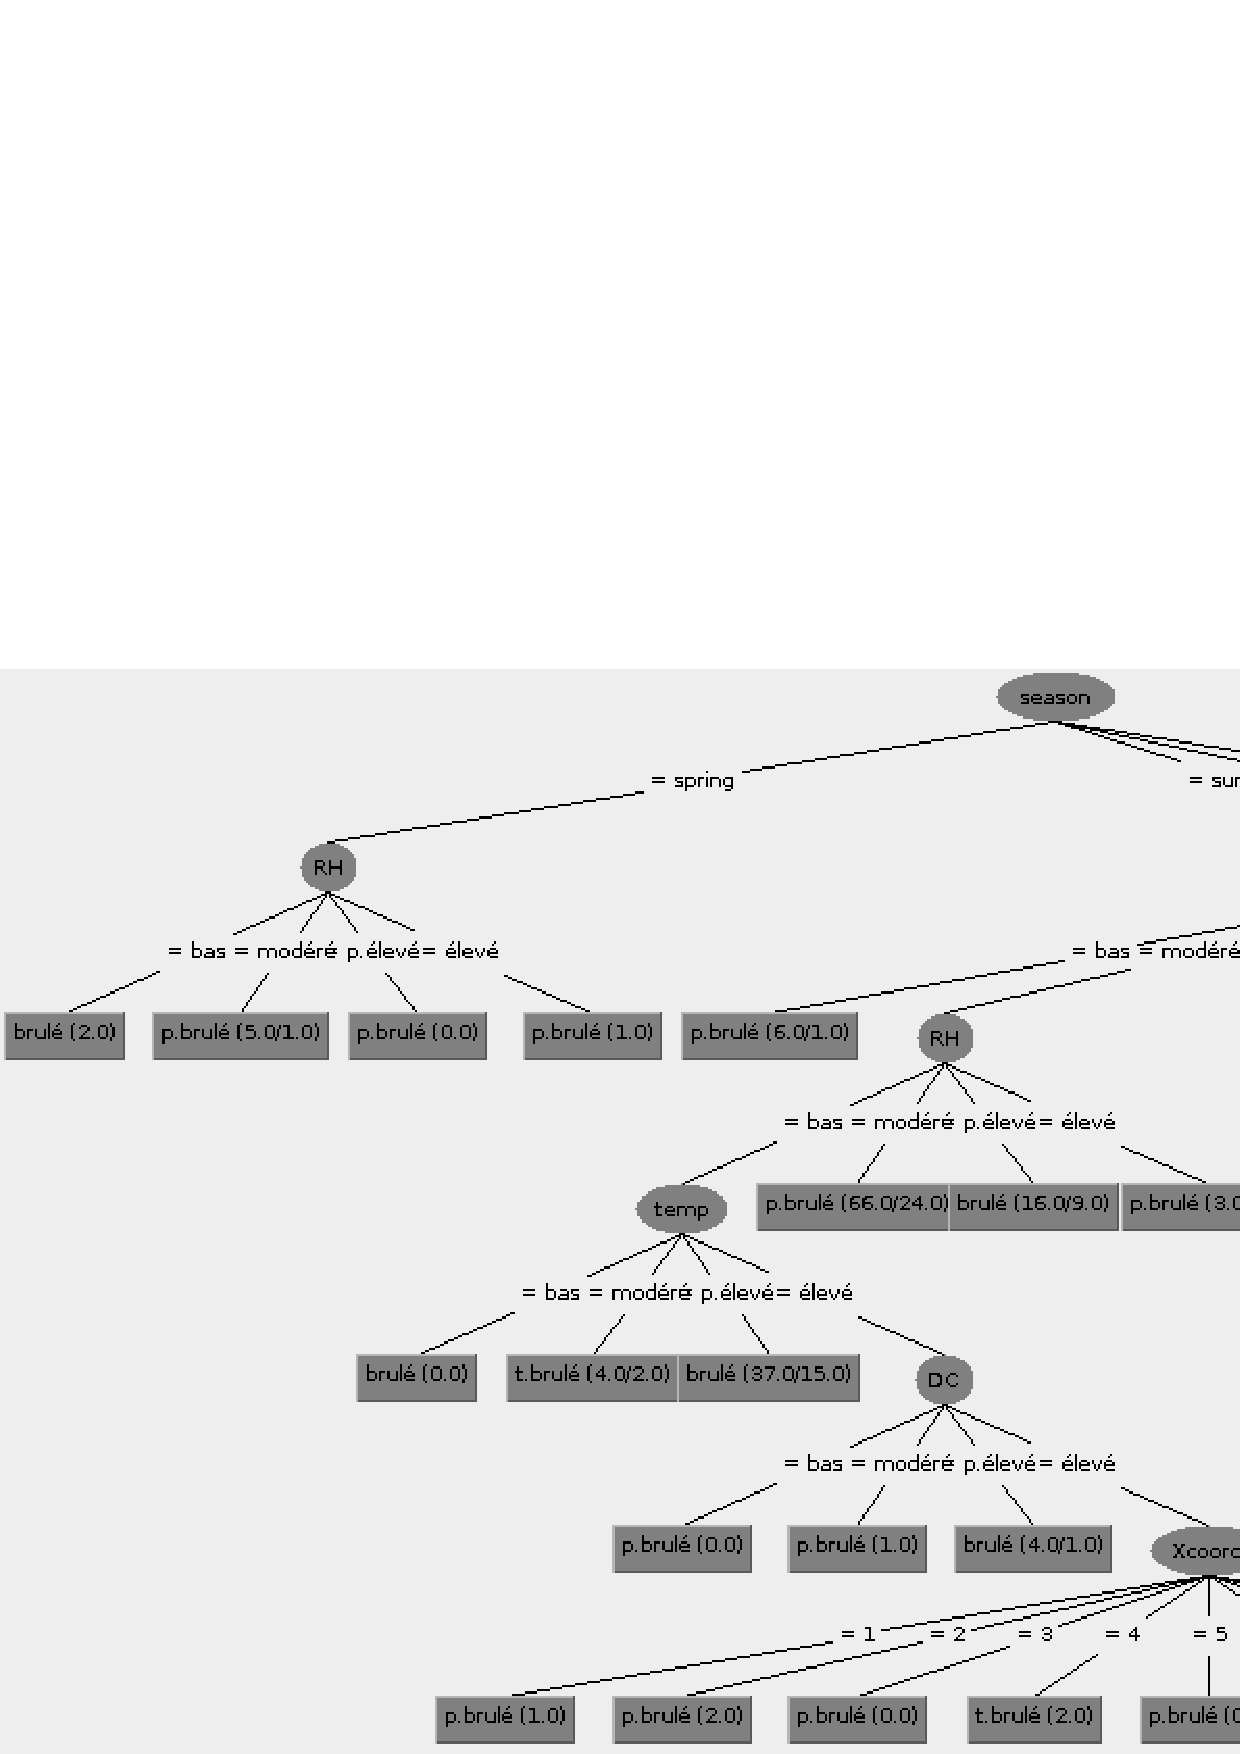
\includegraphics[scale=0.35]{img_005b.pdf}
    \caption{J48 (jeu partiel) :: Arbre}
    \label{j48part}
    \end{center}	
\end{figure}

On peut voir (Figure~\ref{j48part}) que l'algorithme compare tout d'abord la saison pendant laquelle la mesure a été prise, et si
c'est en été il y a beaucoup de paramètre à considérer pour classer les données, sinon vu qu'il y a peu de données, ce que 
l'algorithme trouve n'est pas très probant (même si la classification est logique dans le sens où aucun gros feu n'a lieu en 
hiver, automne ou printemps).\\
Il analyse ensuite les indices du système \textbf{FWI} ainsi que la température afin de classer au mieux possible lorsque la 
saison choisie est l'été. L'arbre a un taux d'erreur assez élevé, ce qui fait qu'il n'est pas très concluant même s'il semble 
confirmer le système \textbf{FWI}.

\subsection{Conclusion de la section}

La classification n'est pas très performante sur le jeu de données, que ce soit l'initial ou le tronqué. Ce n'est pas très étonnant, en effet, les
classes de l'attribut \textbf{area} ne sont pas très bien réparties, dès lors l'algorithme \textit{J48} classe en général un grand nombre d'instance 
dans la classe majoritaire (c'est une bonne chose mais on obtient des résultats pas beaucoup mieux que \textit{ZeroR} et \textit{OneR}) donnant un
taux d'erreur relativement grand (environ $30\%$).

\section{Règles d'association}

Cet outil de weka nous permet de dégager des règles d'association entre différents sous-ensembles d'attributs de la relation. Par 
exemple, on pourrait tirer une règle du genre : $$temp=\text{"t.élevée"} \rightarrow season=\text{"summer"}$$ Bien sûr ce 
genre d'association n'est pas très interessant car elle n'apporte pas de réelles informations, en ce sens où il s'agit d'une 
association de notoriété publique (en effet, s'il fait très chaud alors on est en été en général). \\

L'algorithme utilisé pour cet outil est nommé ``\textbf{Apriori}''. Cet algorithme peut avoir un comportement très différent en 
fonction de 2 paramètres que l'on spécifie : la \textbf{confiance minimale} et le \textbf{support minimum}. La confiance est une 
mesure de qualité sur la règle énoncée tandis que le support permet d'imposer une certaine mesure de couverture minimale des 
données. Ces 2 paramètres sont très importants et complémentaires. En effet la confiance va nous permettre de savoir si la règle 
se vérifie ``souvent'' dans le sens où dès que les prémisses sont rassemblés, on a l'implication qui est vérifiée (dans notre 
exemple : "dès que la température est élevée, on est en été"). Le support quant à lui va nous permettre de sélectionner 
uniquement les règles concernant un nombre minimal d'instances. Effectivement, il est très peu intéressant, par exemple, d'avoir 
des règles, même de confiance égale à 1 (maximum), si seulement 2 instances sur $100.000$ sont concernées.\\

Je vais d'abord appliquer cet algorithme en plaçant la confiance assez basse et le support assez haut, j'augmenterai par la suite
la confiance minimale puis diminuerai le support en fonction du nombre de règles que j'obtiendrai.

\subsection{Dataset initial}

\subsubsection*{Confiance minimale : $0.9$, Support minimal : $0.3$}

Voici les règles trouvées :

\begin{center}
	\begin{boxedverbatim}
Best rules found:
  1. DMC=modéré DC=élevé 158 ==> season=summer 158    conf:(1)
  2. DMC=modéré temp=p.élevé 173 ==> season=summer 168    conf:(0.97)
  3. DMC=modéré ISI=modéré 157 ==> season=summer 152    conf:(0.97)
  4. DMC=modéré 263 ==> season=summer 254    conf:(0.97)
  5. DC=élevé temp=p.élevé 168 ==> season=summer 161    conf:(0.96)
  6. DMC=modéré area=p.brulé 190 ==> season=summer 182    conf:(0.96)
  7. DC=élevé area=p.brulé 190 ==> season=summer 180    conf:(0.95)
  8. DC=élevé 274 ==> season=summer 259    conf:(0.95)
  9. FFMC=élevé 217 ==> season=summer 205    conf:(0.94)
 10. DC=élevé ISI=modéré 165 ==> season=summer 154    conf:(0.93)
 11. temp=p.élevé 257 ==> season=summer 238    conf:(0.93)
 12. temp=p.élevé area=p.brulé 186 ==> season=summer 172    conf:(0.92)	
	\end{boxedverbatim}
\end{center}

La première observation que l'on peut faire est que toutes les règles trouvées concernent l'attribut \textbf{season} prenant la 
valeur \textit{summer}. C'est pas très étonnant, en effet, plus de $75\%$ des données ont la valeur \textit{summer} pour 
l'attribut \textbf{season}. Parmi les règles trouvées, certaines sont peu utiles du fait qu'elles sont totalement logiques, en 
effet, par exemple, la règle précédemment énoncée à titre d'exemple se retrouve dans les résultats (bien que la température soit
égale à ``peu élevée'', mais c'est compréhensible vu que la majorité des données ont celle valeur pour la température). \\

On peut néanmoins remarquer qu'avoir un indice \textbf{DMC} modéré et un indice \textbf{DC} élevé implique à coup sur que la saison pendant
laquelle les mesures ont été prises est l'été. Aussi, un \textbf{DMC} modéré, un \textbf{DC} élevé ou un \textbf{FFMC} élevé implique en général que 
les mesures ont été prises en été. Mais encore, un feu bénin associé à une température un peu élevée, un \textbf{DMC} modéré ou un 
\textbf{DC} élevé implique que les mesures ont été prises en été.\\
Il faut relativiser, en effet, comme dit dans la section de la classification, 
beaucoup de données ont la valeur \textit{``peu brulée''} pour l'attribut \textbf{area}. Ce fut d'ailleurs mon argument pour tronquer un peu le jeu 
de données. Il faut tout de même rappeller que les données sont à chaque fois des feux de forêts, c'est-à-dire que bien que ce soit la saison qui 
soit concernée à chaque fois, il n'en reste néanmoins que cela concerne également des feux de forêts de gravités variées. Ainsi on peut conclure de 
ces premières règles que les situations suivantes correspondent à un risque élevé d'un feu de forêt : 
\begin{itemize}
\item une combinaison (de $1$, $2$ ou $3$ éléments) d'un \textbf{ISI} modéré, \textbf{DMC} modéré ou \textbf{DC} élevé,
\item un \textbf{DMC} modéré et une température un peu élevée,
\item un \textbf{FFMC} élevé,
\item un \textbf{DC} élevé et une température un peu élevée.
\end{itemize}

\subsubsection*{Confiance minimale : $0.9$, Support minimal : $0.2$}

Dans cette configuration, avec une limitation du nombre de règles trouvées à $100$, l'algorithme trouve $50$ règles. Pour des soucis de lisibilité 
ces règles ne sont pas données ici (elles sont disponibles dans l'annexe~\ref{annexA} cependant). \\

Mis à part les règles déjà trouvées précédemment, on en tire quelques nouvelles qui peuvent être intéressantes :
\begin{itemize}
\item en week-end, si le \textbf{DMC} est modéré (ou le \textbf{DC} élevé ou la température peu élevée), risque d'incendie. Cette règle aussi bénine 
puisse-t-elle sembler permet de confirmer une influence 
de l'homme sur les incendies (la majeure partie de ceux-ci étant d'origine humaine).
\item si le \textbf{FFMC} est élevé et que le vent est modéré, risque d'incendie. Assez logique, le vent souffle assez fort pour attiser le feu et 
lui permettre de s'étendre un tant soit peu mais pas assez pour l'éteindre.
\item si on se trouve en ``$y=4$'' et le \textbf{DMC} est modéré (ou le \textbf{DC} élevé ou la température peu élevée), risque d'incendie. Cette 
règle est à relativiser car $y=4$ correspond à l'ordonnée pour laquelle le découpage couvre le mieux le parc, il est donc logique qu'il y ait plus 
d'incendies dans ces cases qu'ailleurs. Celà dit, si on regarde sur une carte physique 
\footnote{http://www.globeholidays.net/Europe/Portugal/Tras\_Montes\_Alto\_Douro/Montesinho/Maps2.htm}, on remarque qu'il y a pas mal de villages sur 
ces ordonnées ainsi que des espaces verts, ce n'est pas donc pas étonnant que l'on déplore autant de feux à ces endroits.

\end{itemize}

\subsubsection*{Confiance minimale : $0.7$, Support minimal : $0.2$}

Dans cette configuration, avec une limitation du nombre de règles trouvées à $100$, l'algorithme trouve $100$ règles. Pour des soucis de lisibilité 
ces règles ne sont pas données ici (elles sont disponibles dans l'annexe~\ref{annexB} cependant). \\

Ici on trouve d'autres règles qui n'impliquent pas toutes l'attribut \textbf{season} avec la valeur \textit{summer} :
\begin{center}
	\begin{verbatim}
 55. season=summer RH=bas 139 ==> FFMC=élevé 110    conf:(0.79)
 67. season=summer RH=modéré 169 ==> area=p.brulé 128    conf:(0.76)
 70. RH=modéré 221 ==> area=p.brulé 165    conf:(0.75)
 72. YCoord=4 season=summer 154 ==> area=p.brulé 114    conf:(0.74)
 73. temp=modéré 158 ==> area=p.brulé 116    conf:(0.73)
 75. DMC=modéré ISI=modéré 157 ==> area=p.brulé 115    conf:(0.73)
 77. season=summer DMC=modéré ISI=modéré 152 ==> area=p.brulé 111    conf:(0.73)
 79. FFMC=élevé DC=élevé 144 ==> area=p.brulé 105    conf:(0.73)
 80. season=summer RH=modéré 169 ==> temp=p.élevé 123    conf:(0.73)
 81. ISI=modéré temp=p.élevé 143 ==> area=p.brulé 104    conf:(0.73)
 82. season=summer FFMC=p.élevé 167 ==> area=p.brulé 121    conf:(0.72)
 83. temp=p.élevé 257 ==> area=p.brulé 186    conf:(0.72)
 84. season=summer FFMC=élevé DC=élevé 141 ==> area=p.brulé 102    conf:(0.72)
 85. season=summer temp=p.élevé 238 ==> area=p.brulé 172    conf:(0.72)
 86. DMC=modéré temp=p.élevé 173 ==> area=p.brulé 125    conf:(0.72)
 87. DMC=modéré 263 ==> area=p.brulé 190    conf:(0.72)
 88. season=summer ISI=modéré area=p.brulé 154 ==> DMC=modéré 111    conf:(0.72)
 89. FFMC=p.élevé 229 ==> area=p.brulé 165    conf:(0.72)
 90. season=summer day=weekday 189 ==> area=p.brulé 136    conf:(0.72)
 91. season=summer DMC=modéré ISI=modéré 152 ==> DC=élevé 109    conf:(0.72)
 92. season=summer DMC=modéré 254 ==> area=p.brulé 182    conf:(0.72)
 93. YCoord=4 197 ==> area=p.brulé 141    conf:(0.72)
 94. season=summer DMC=modéré temp=p.élevé 168 ==> area=p.brulé 120    conf:(0.71)
 95. ISI=modéré temp=p.élevé 143 ==> DMC=modéré 102    conf:(0.71)
 96. season=summer FFMC=élevé area=p.brulé 143 ==> DC=élevé 102    conf:(0.71)
 97. season=summer FFMC=élevé DMC=modéré 142 ==> area=p.brulé 101    conf:(0.71)
 98. season=summer RH=modéré 169 ==> DMC=modéré 120    conf:(0.71)
 99. ISI=modéré 268 ==> area=p.brulé 190    conf:(0.71)
100. FFMC=élevé DMC=modéré 144 ==> area=p.brulé 102    conf:(0.71)
	\end{verbatim}
\end{center}

La plupart concerne l'attribut \textbf{area} avec la valeur \textit{peu brulée}, ce qui, à nouveau, est compréhensible vu que la grande majorité des 
données possède cette valeur pour cet attribut. On ne peut donc pas tirer beaucoup d'informations de ces règles mis à part le fait qu'en été (et donc 
toutes les situations décrites plus haut) un peu plus de $70\%$ des feux de forêts sont "benins". Cette information étant visible via la 
visualisation disponible au début du rapport, elle n'est donc pas très importante. Il y a cependant quelques règles que l'on peut voir apparaître et 
qui peuvent être interessantes :
\begin{center}
	\begin{boxedverbatim}
 55. season=summer RH=bas 139 ==> FFMC=élevé 110    conf:(0.79)
 91. season=summer DMC=modéré ISI=modéré 152 ==> DC=élevé 109    conf:(0.72)
 95. ISI=modéré temp=p.élevé 143 ==> DMC=modéré 102    conf:(0.71)
 98. season=summer RH=modéré 169 ==> DMC=modéré 120    conf:(0.71)
	\end{boxedverbatim}
\end{center}

On apprend ainsi que dans $80\%$ des cas où le \textbf{RH} est bas en été, le \textbf{FFMC} est élevé. Celà peut être utile si on ne peut pour des 
raisons diverses (budgetaires, techniques, ...) mesurer le \textbf{FFMC} en été, en effet, on pourra déduire sur base d'une erreur de $20\%$ et que 
le \textbf{RH} est bas que le \textbf{FFMC} est élevé. Il en va de même pour les autres règles ci-dessus avec des taux d'erreur plus important 
cependant. \\

A part quelque relation entre les indices, la température et le vent sur le fait qu'il y a un feu ou pas, je n'ai pas pu retirer beaucoup 
d'informations de ce jeu de données. Je vais donc essayer de raffiner en enlevant toutes les instances dont la valeur pour l'attribut \textbf{season}
est \textit{summer}. J'obtiens ainsi un dataset assez pauvre avec seulement $122$ instances, il conviendra donc d'être prudent sur les règles 
énoncées par l'algorithme. Je place le support assez haut et la confiance pas spécialement haute (0.5 et 0.7) afin d'avoir des règles vraiment 
plausibles au vu du faible nombre d'instances. L'algorithme donne :

\begin{center}
	\begin{boxedverbatim}
  1. DC=bas 82 ==> DMC=bas 82    conf:(1)
  2. season=winter 71 ==> DMC=bas 71    conf:(1)
  3. season=winter DC=bas 70 ==> DMC=bas 70    conf:(1)
  4. season=winter 71 ==> DC=bas 70    conf:(0.99)
  5. season=winter DMC=bas 71 ==> DC=bas 70    conf:(0.99)
  6. season=winter 71 ==> DMC=bas DC=bas 70    conf:(0.99)
  7. temp=modéré 70 ==> DMC=bas 67    conf:(0.96)
  8. area=p.brulé 83 ==> DMC=bas 73    conf:(0.88)
  9. DC=bas 82 ==> season=winter 70    conf:(0.85)
 10. DMC=bas DC=bas 82 ==> season=winter 70    conf:(0.85)
 11. DC=bas 82 ==> season=winter DMC=bas 70    conf:(0.85)
 12. DMC=bas 111 ==> DC=bas 82    conf:(0.74)
	\end{boxedverbatim}
\end{center}

Les 6 premières règles ainsi que les règles de 9 à 12 relatent une relation forte entre la saison hivernale, le \textbf{DMC} bas et le \textbf{DC} 
bas, connaître un de ces 3 paramètres permettrait de connaître les 2 autres. Ainsi, si on se trouve en hiver, le \textbf{DMC} et le \textbf{DC} sont 
bas ou encore si on sait que le \textbf{DMC} est bas alors on est en saison hivernale. La 7ème règle est un peu redondante, bien que plus générale 
que la 2ème, en effet, en hiver la température est majoritairement ``modérée''. La règle 8 peut paraître perturbante au premier abord, en effet, elle 
dit implicitement que si un feu peu important a eu lieu, alors il a eu lieu en hiver, saison où normalement très peu de feux devraient avoir lieu. 
Cependant, il ne faut pas oublier que dans ce parc il y a des villages habités, il faut donc que les gens se chauffent, il se peut donc que les feux 
soient initiés par des feux de cheminées, ou un feu dans un jardin ...

\subsection{Conclusion de la section}

Je n'ai pas pu utiliser les informations données pour déterminer la gravité du feu, cependant j'ai pu mettre à vue certaines conditions pour 
lesquelles le risque de feu est élevé. J'ai également mis en évidence certaines relations entre les valeurs des indices du système \textbf{FWI}, il 
se peut donc que pour certaines valeurs de ces indices, certains sont redondants et donc inutiles à calculer.

\newpage

\section{Clustering}

Ce dernier outil de weka que je vais utiliser consiste à regrouper les données \textit{``proches''} (au sens d'une certaine norme, à définir) en 
groupe, afin d'obtenir des informations supplémentaires. 2 algorithmes sont à notre disposition : \textbf{SimpleKMeans} et \textbf{EM}. Je vais 
d'abord utiliser \textbf{EM} car il permet de deviner le nombre de groupes normalement optimal pour le clustering. Par la suite nous appliquerons 
\textbf{SimpleKMeans} avec le nombre trouvé par \textbf{EM} afin d'affiner la recherche.

\subsection{EM}

\textbf{EM} propose $9$ clusters :

\begin{center}
	\begin{boxedverbatim}
Clustered Instances

0      103 ( 20%)
1       50 ( 10%)
2      132 ( 26%)
3       42 (  8%)
4       16 (  3%)
5       31 (  6%)
6       36 (  7%)
7       53 ( 10%)
8       42 (  8%)
	\end{boxedverbatim}
\end{center}

J'ai décidé d'ignorer les coordonnées pour cette analyse, car elles n'apportent pas beaucoup d'informations. Je vais à présent montrer les 
représentations de chaque attributs en fonction des clusters, commenter ces représentations et au final essayer d'obtenir des informations au vu du
regroupement fait par l'algorithme.

\begin{figure}[h!]
    \begin{center}
    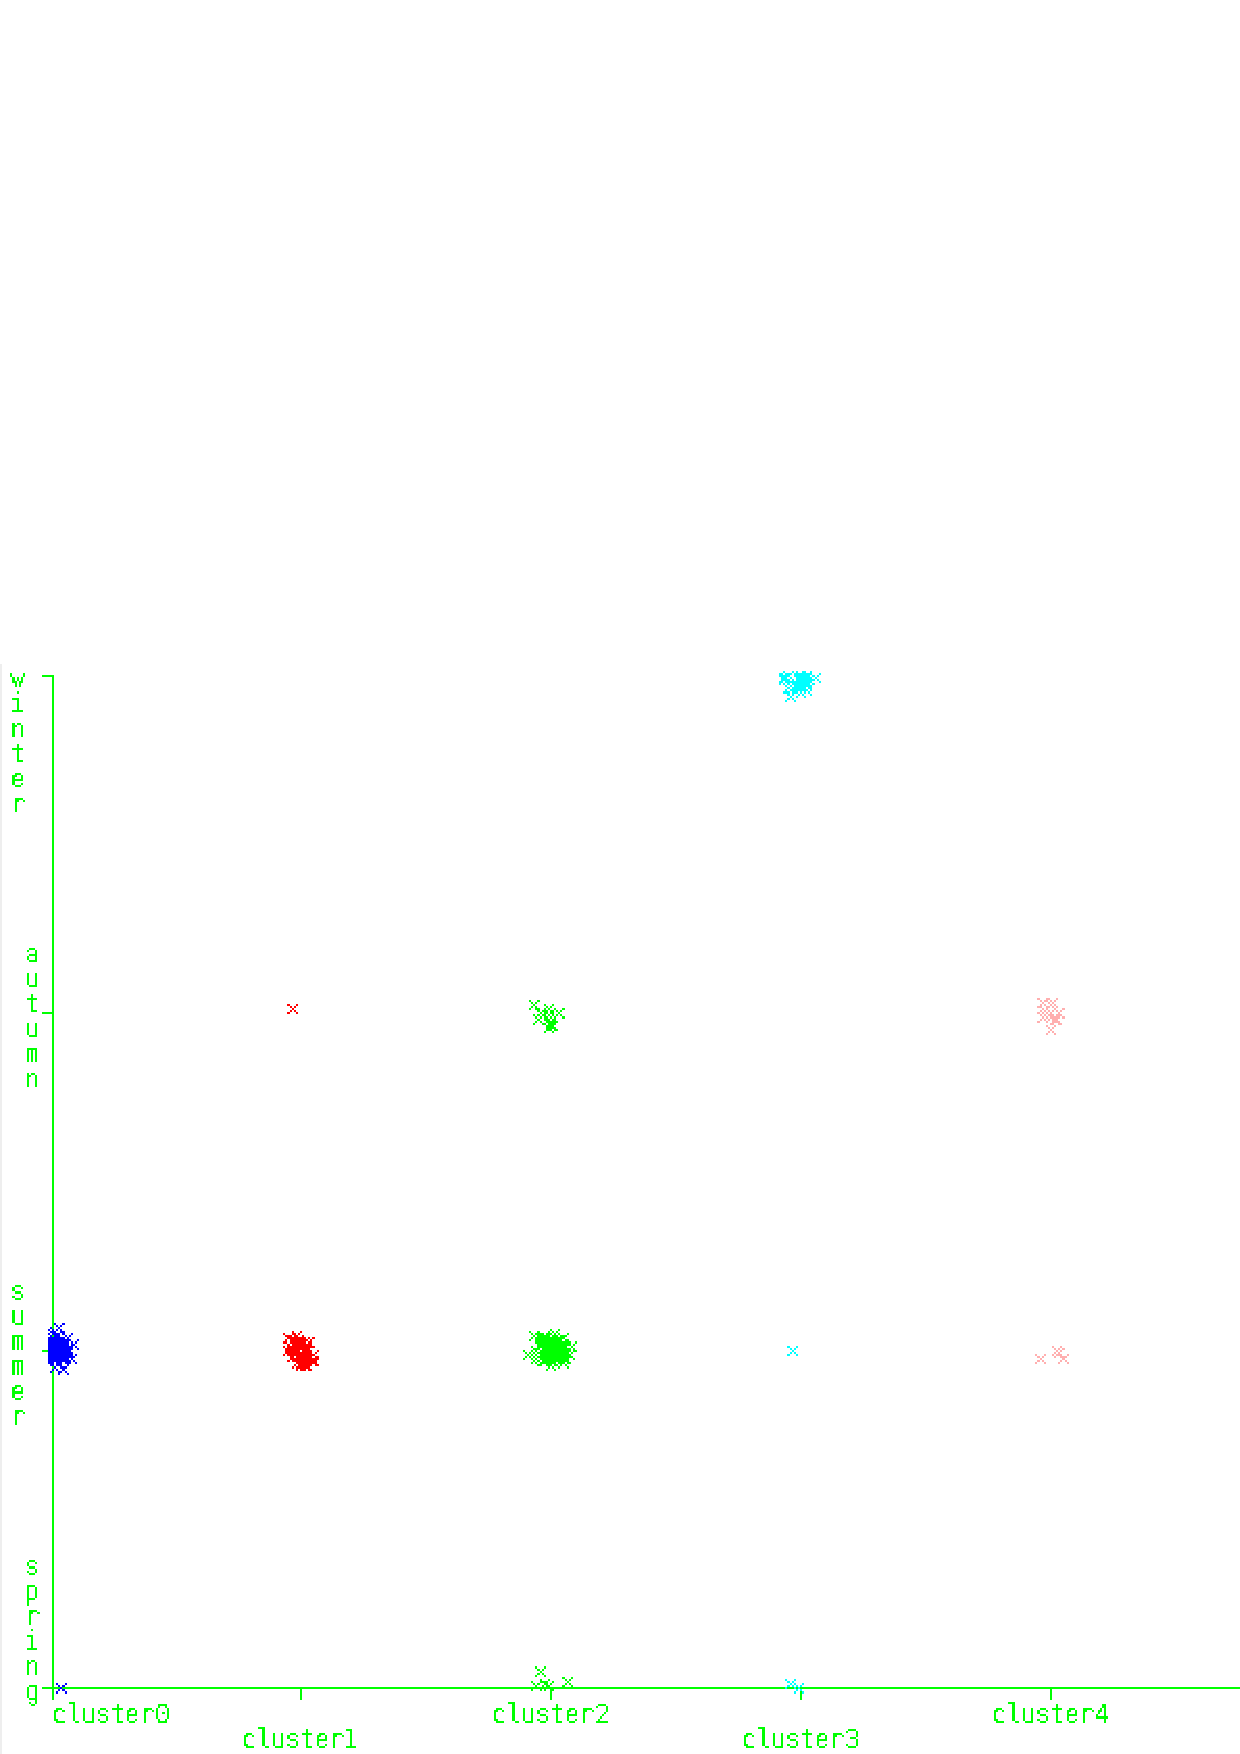
\includegraphics[width=\textwidth]{img_007.pdf}
    \caption{Clusters/season}
    \end{center}	
\end{figure}

Sur ce graphe on remarque que les clusters sont assez bien répartis, en effet les clusters $0$, $1$, $2$, $5$, $6$ et $7$ regroupent une grande 
majorité de valeur \textit{summer} tandis que les clusters $3$ et $8$ regroupent les valeurs \textit{winter} et le cluster $4$ les valeurs 
\textit{autumn}. Seule la valeur \textit{spring} n'est pas vraiment concentrée dans un cluster.

\newpage

\begin{figure}[h!]
    \begin{center}
    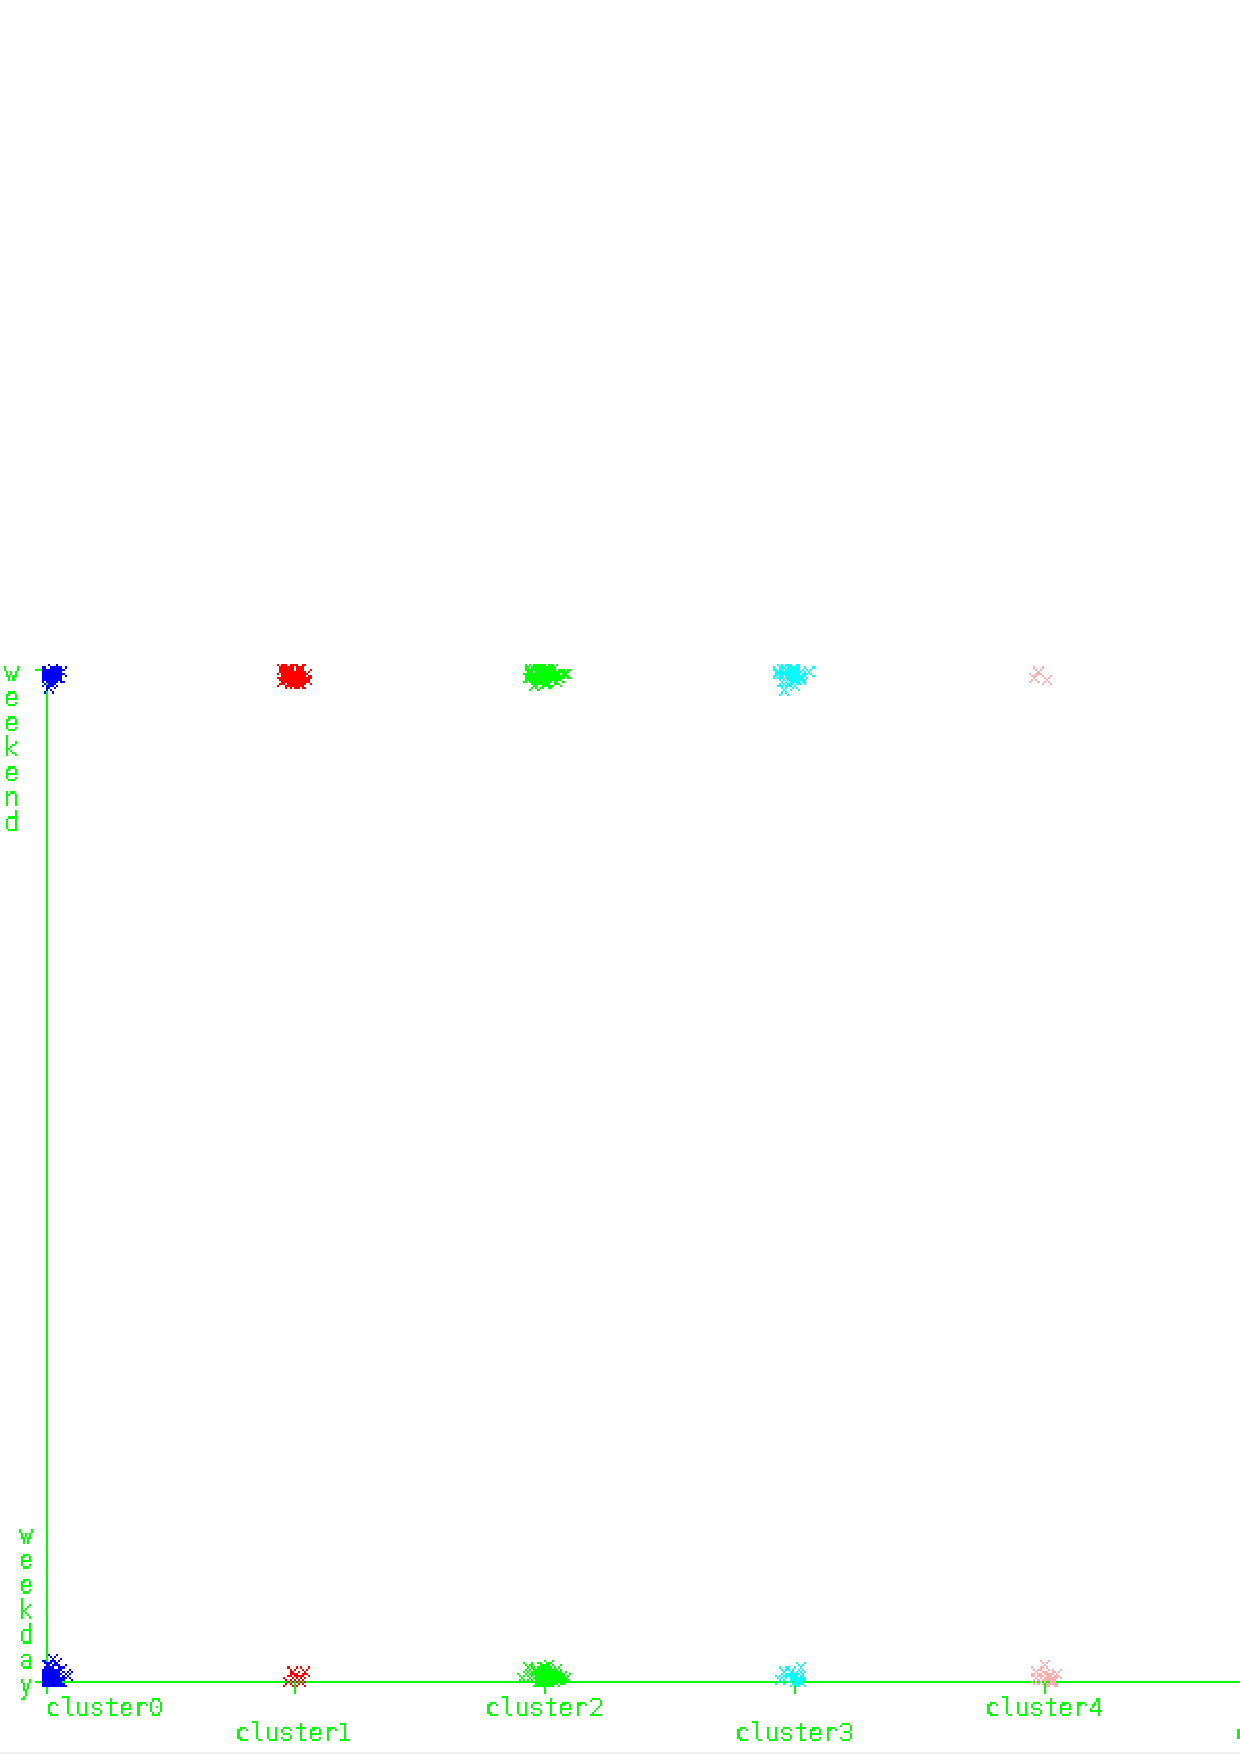
\includegraphics[width=\textwidth]{img_008.pdf}
    \caption{Clusters/day}
    \end{center}	
\end{figure}

Pour l'attribut \textbf{day}, rien d'interessant mis à part peut-être le cluster $1$ qui contient majoritairement des valeurs \textit{week-end} et 
le cluster $4$ des valeurs \textit{weekday} mais rien de bien probant.

\begin{figure}[h!]
    \begin{center}
    \includegraphics[width=\textwidth]{img_009.pdf}
    \caption{Clusters/FFMC}
    \end{center}	
\end{figure}

Ici le découpage est assez interessant,
\begin{itemize}
\item clusters $0$ et $7$ $\rightarrow$ \textbf{FFMC} élevé
\item clusters $1$, $2$, $3$ et $6$ $\rightarrow$ \textbf{FFMC} un peu élevé
\item clusters $4$, $5$ et $8$ $\rightarrow$ \textbf{FFMC} modéré
\end{itemize}
\newpage
\begin{figure}[h!]
    \begin{center}
    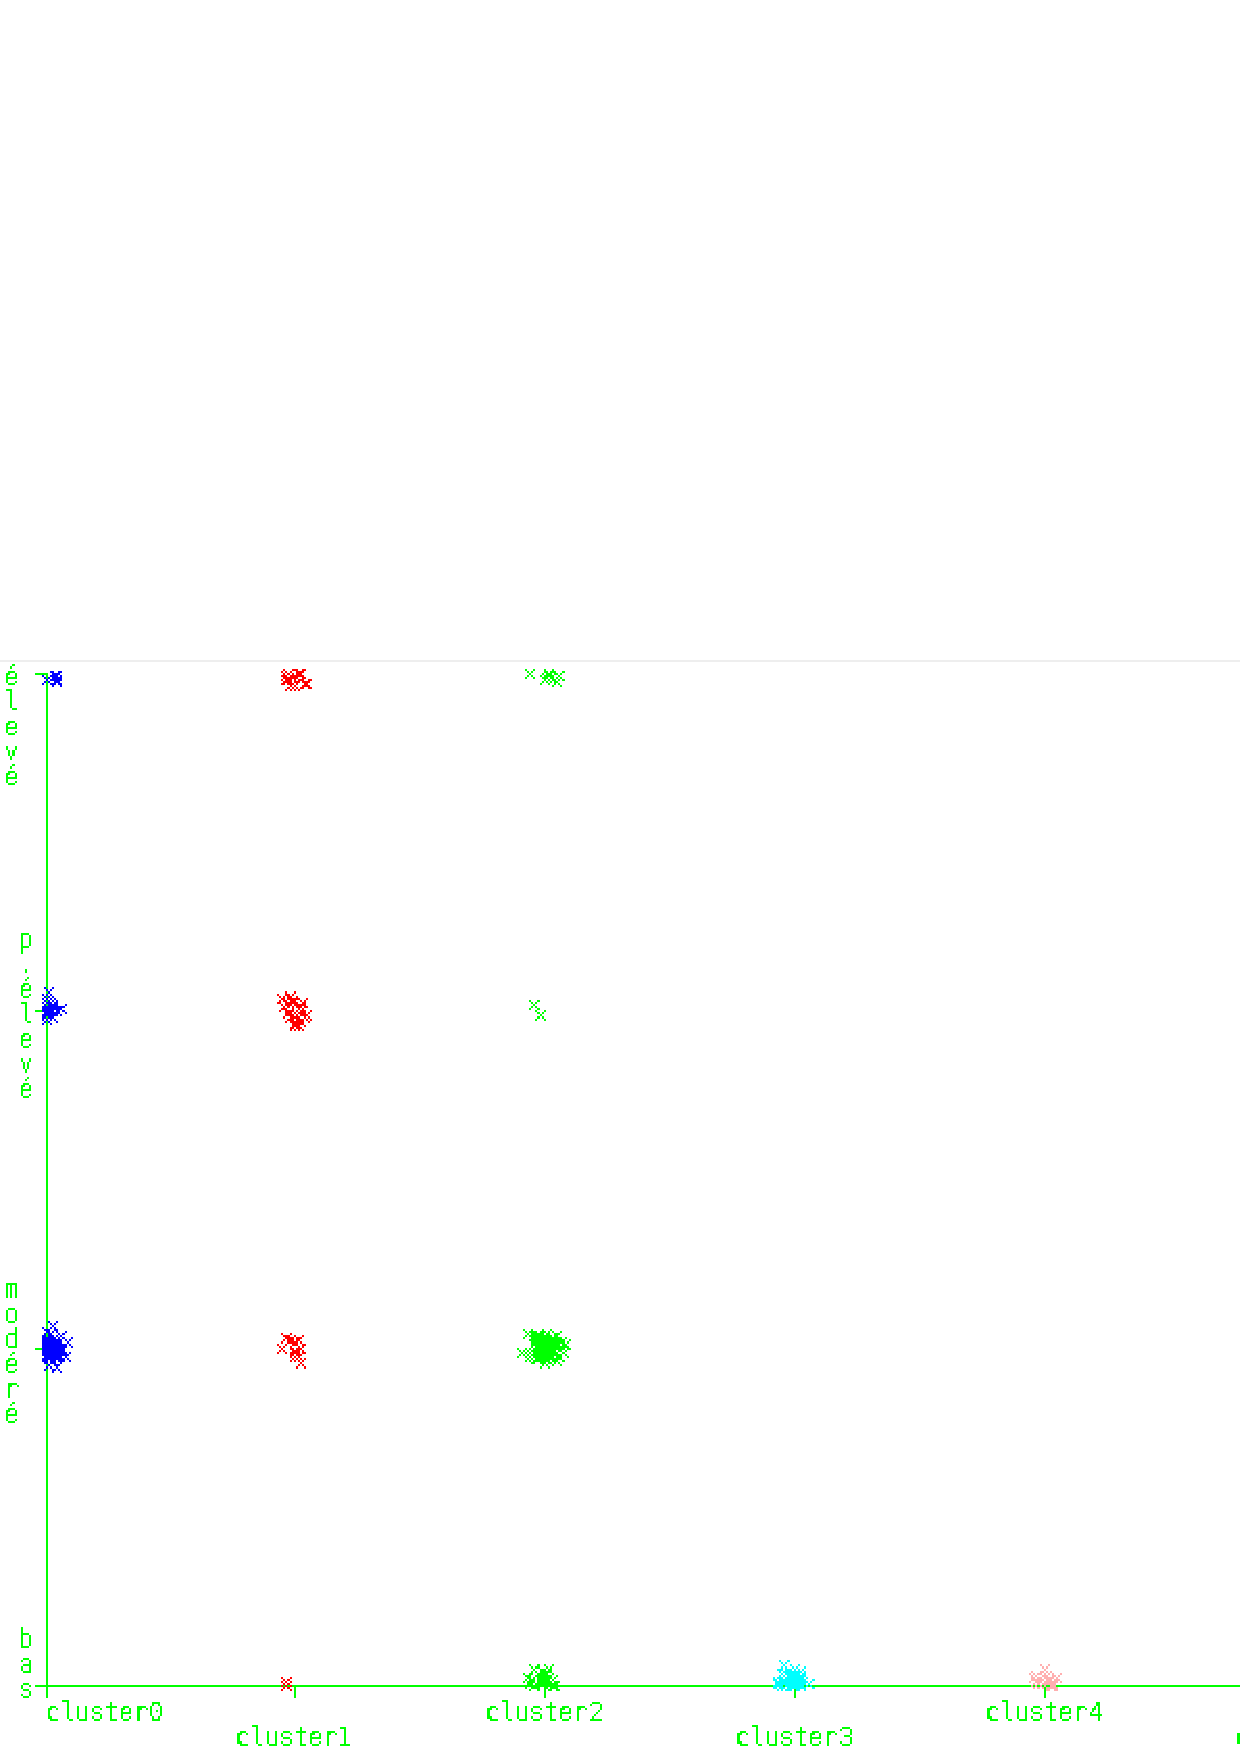
\includegraphics[width=\textwidth]{img_010.pdf}
    \caption{Clusters/DMC}
    \end{center}	
\end{figure}

Ici, le cluster $0$ contient des valeurs \textit{modéré} ou supérieure, les clusters $3$, $4$ et $8$ que des valeurs \textit{bas}. Les autres 
clusters sont assez disparates. On pourait alors pratiquement classer les clusters ici en \textit{``bas''} et \textit{''pas bas''}.

\begin{figure}[h!]
    \begin{center}
    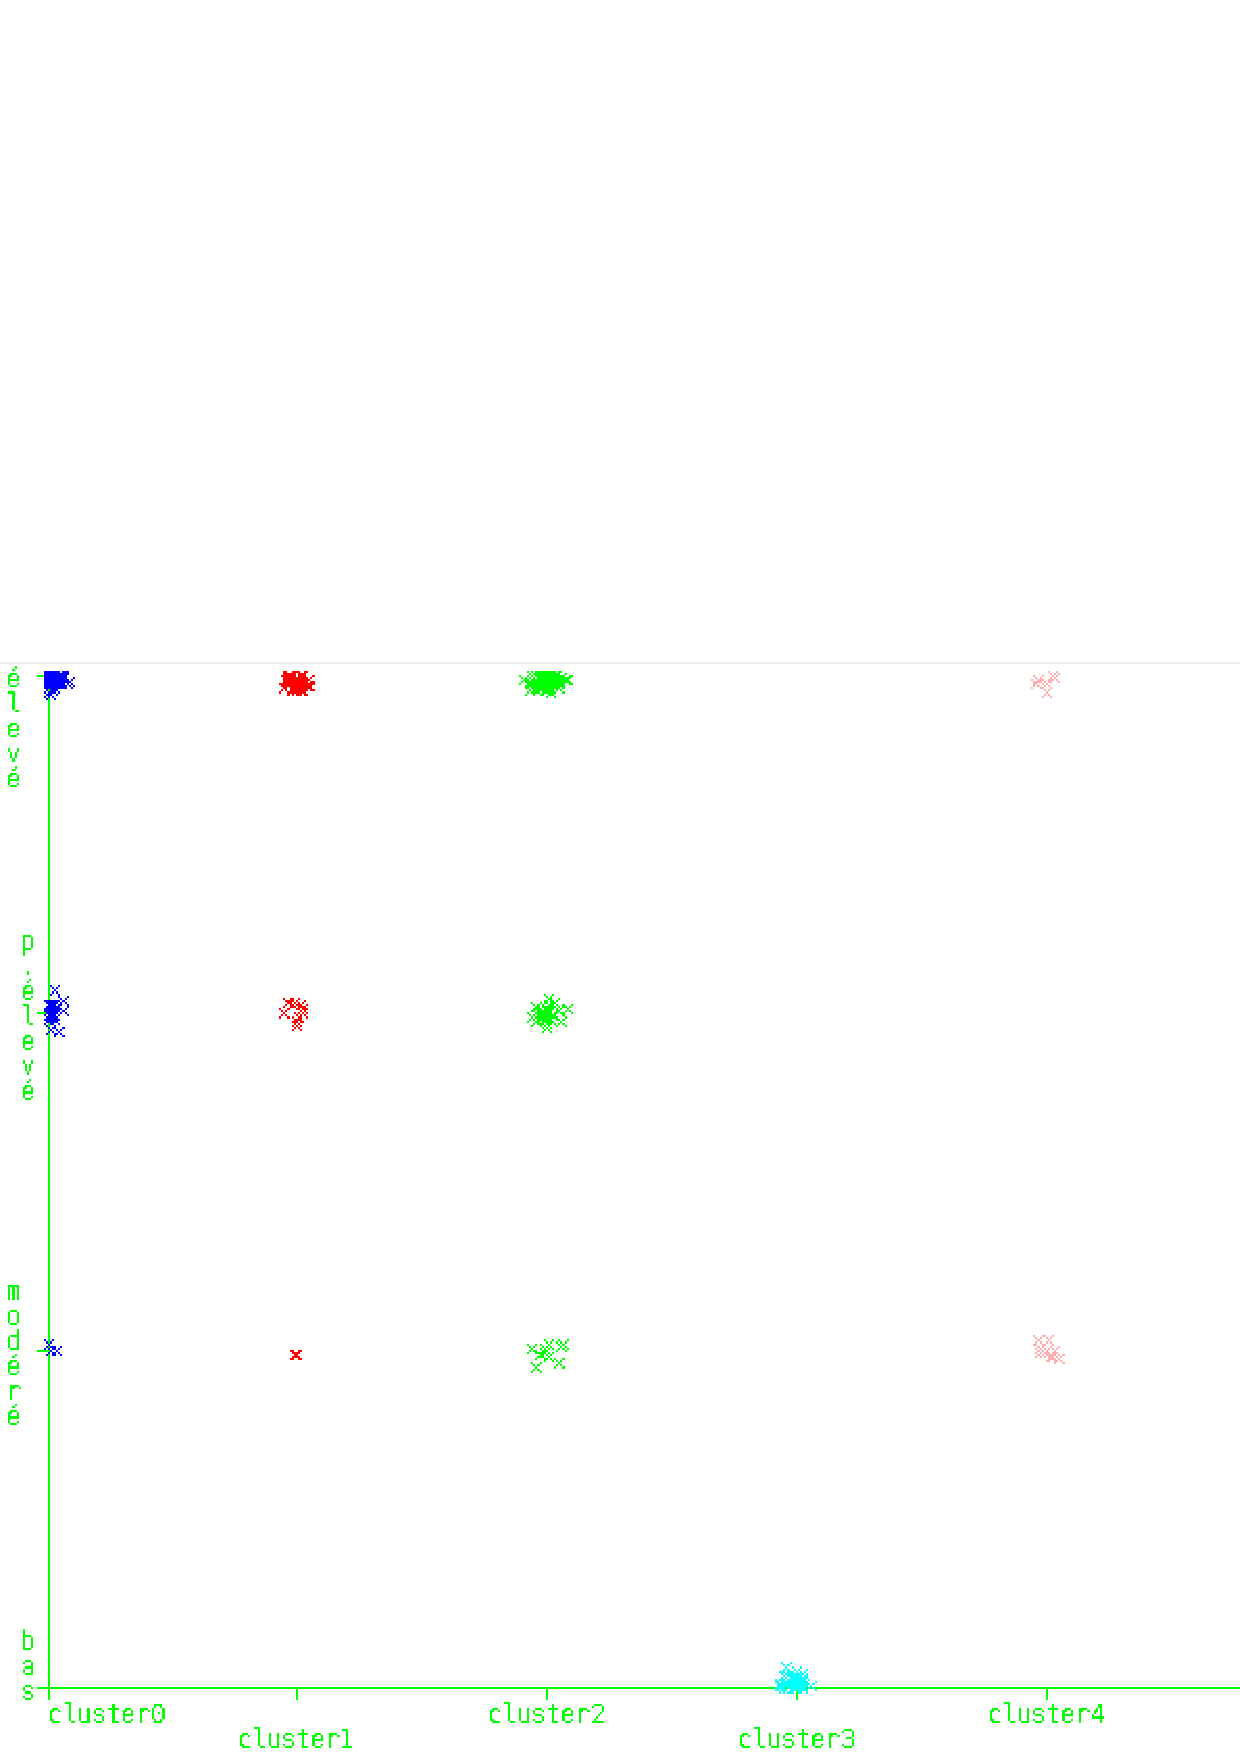
\includegraphics[width=\textwidth]{img_011.pdf}
    \caption{Clusters/DC}
    \end{center}	
\end{figure}

De manière semblable à \textbf{DMC}, les clusters $3$ et $8$ ne contiennent que des valeurs \textit{bas} tandis que les autres n'en contiennent pas. 
On pourrait alors les classer de la même manière en \textit{``bas''} et \textit{``pas bas''}.
\newpage
\begin{figure}[h!]
    \begin{center}
    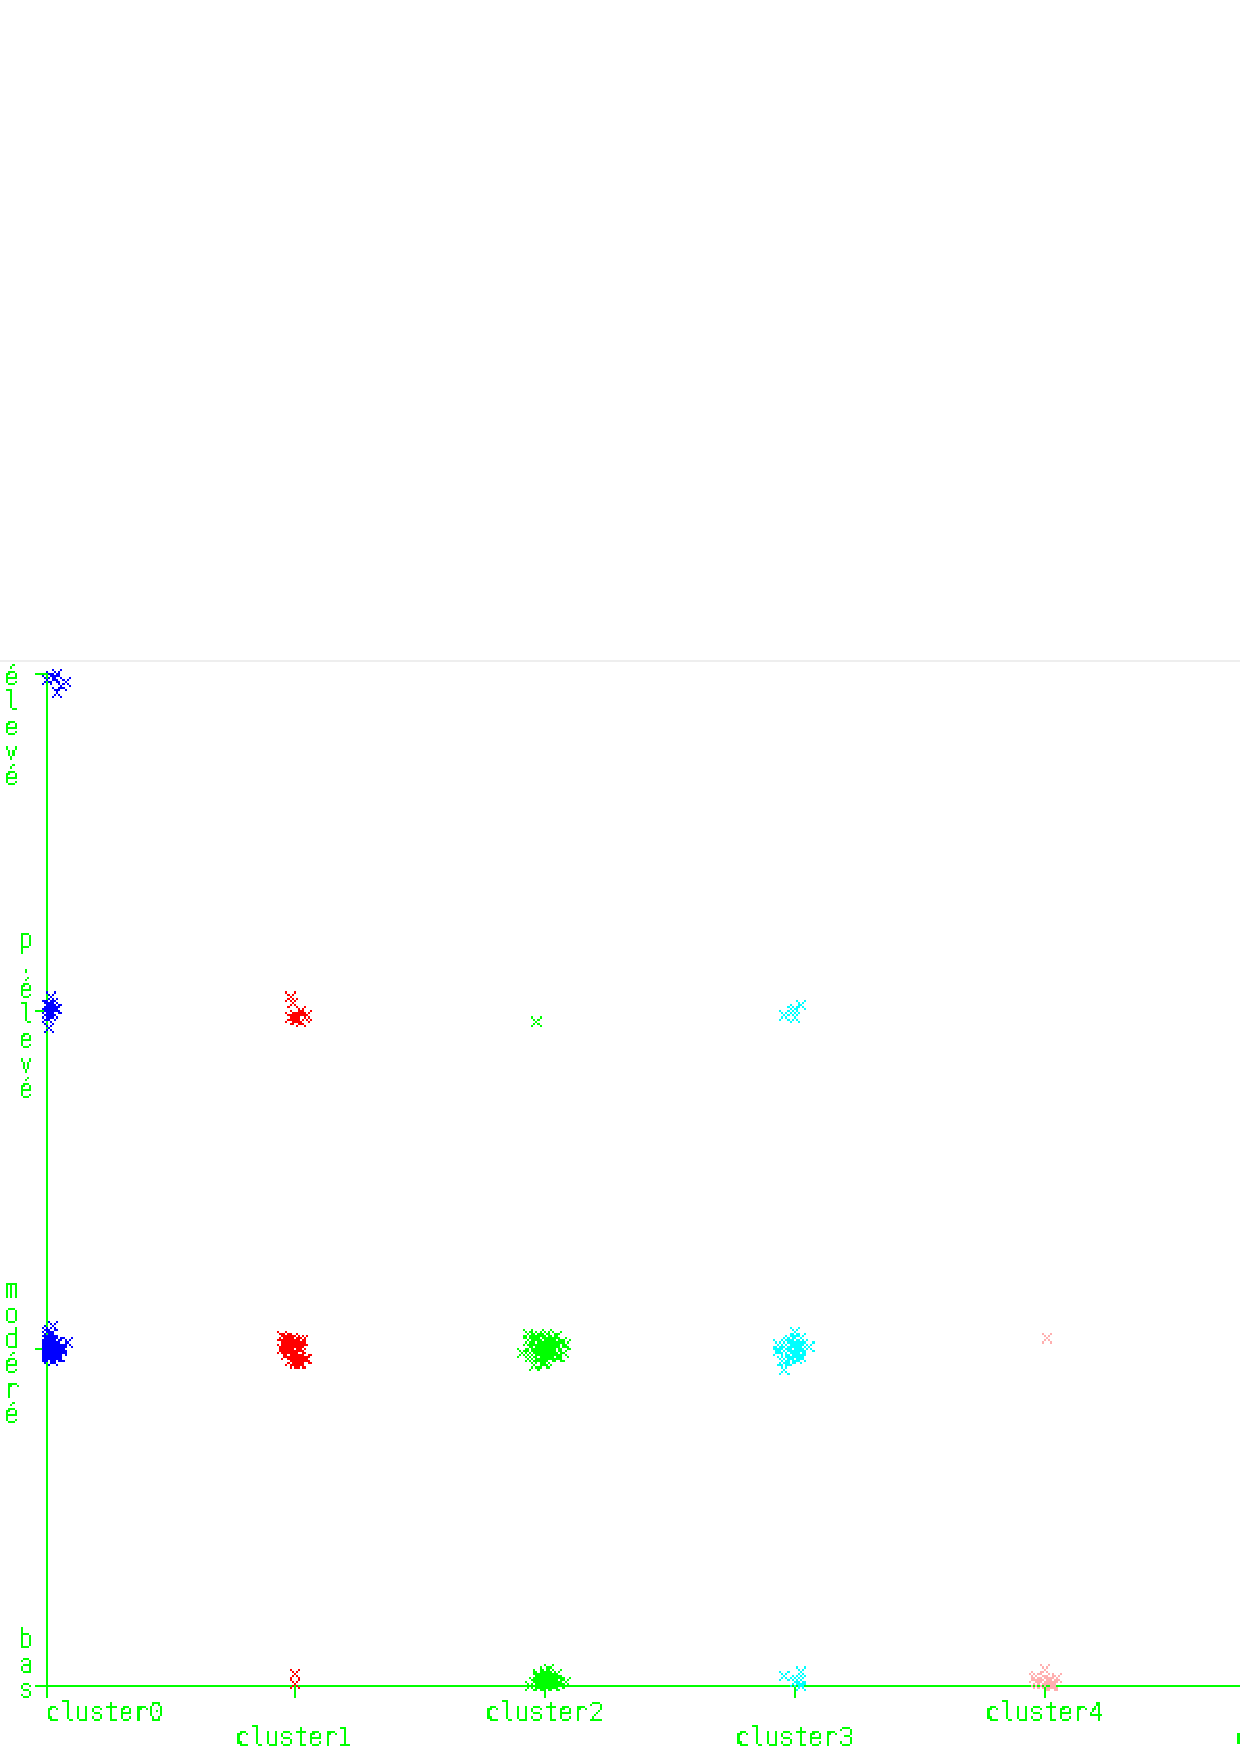
\includegraphics[width=\textwidth]{img_012.pdf}
    \caption{Clusters/ISI}
    \end{center}	
\end{figure}

Les clusters $0$ et $7$ contient des valeurs \textit{modéré} ou supérieure, les clusters $4$ et $8$ des valeurs \textit{bas}. Les clusters $1$ et $3$ 
des valeurs \textit{modéré} principalement tandis que le cluster $2$ des données \textit{bas} ou \textit{modéré}. Finalement le cluster $5$ contient 
des valeurs \textit{modéré} ou \textit{un peu élevée}.

\begin{figure}[h!]
    \begin{center}
    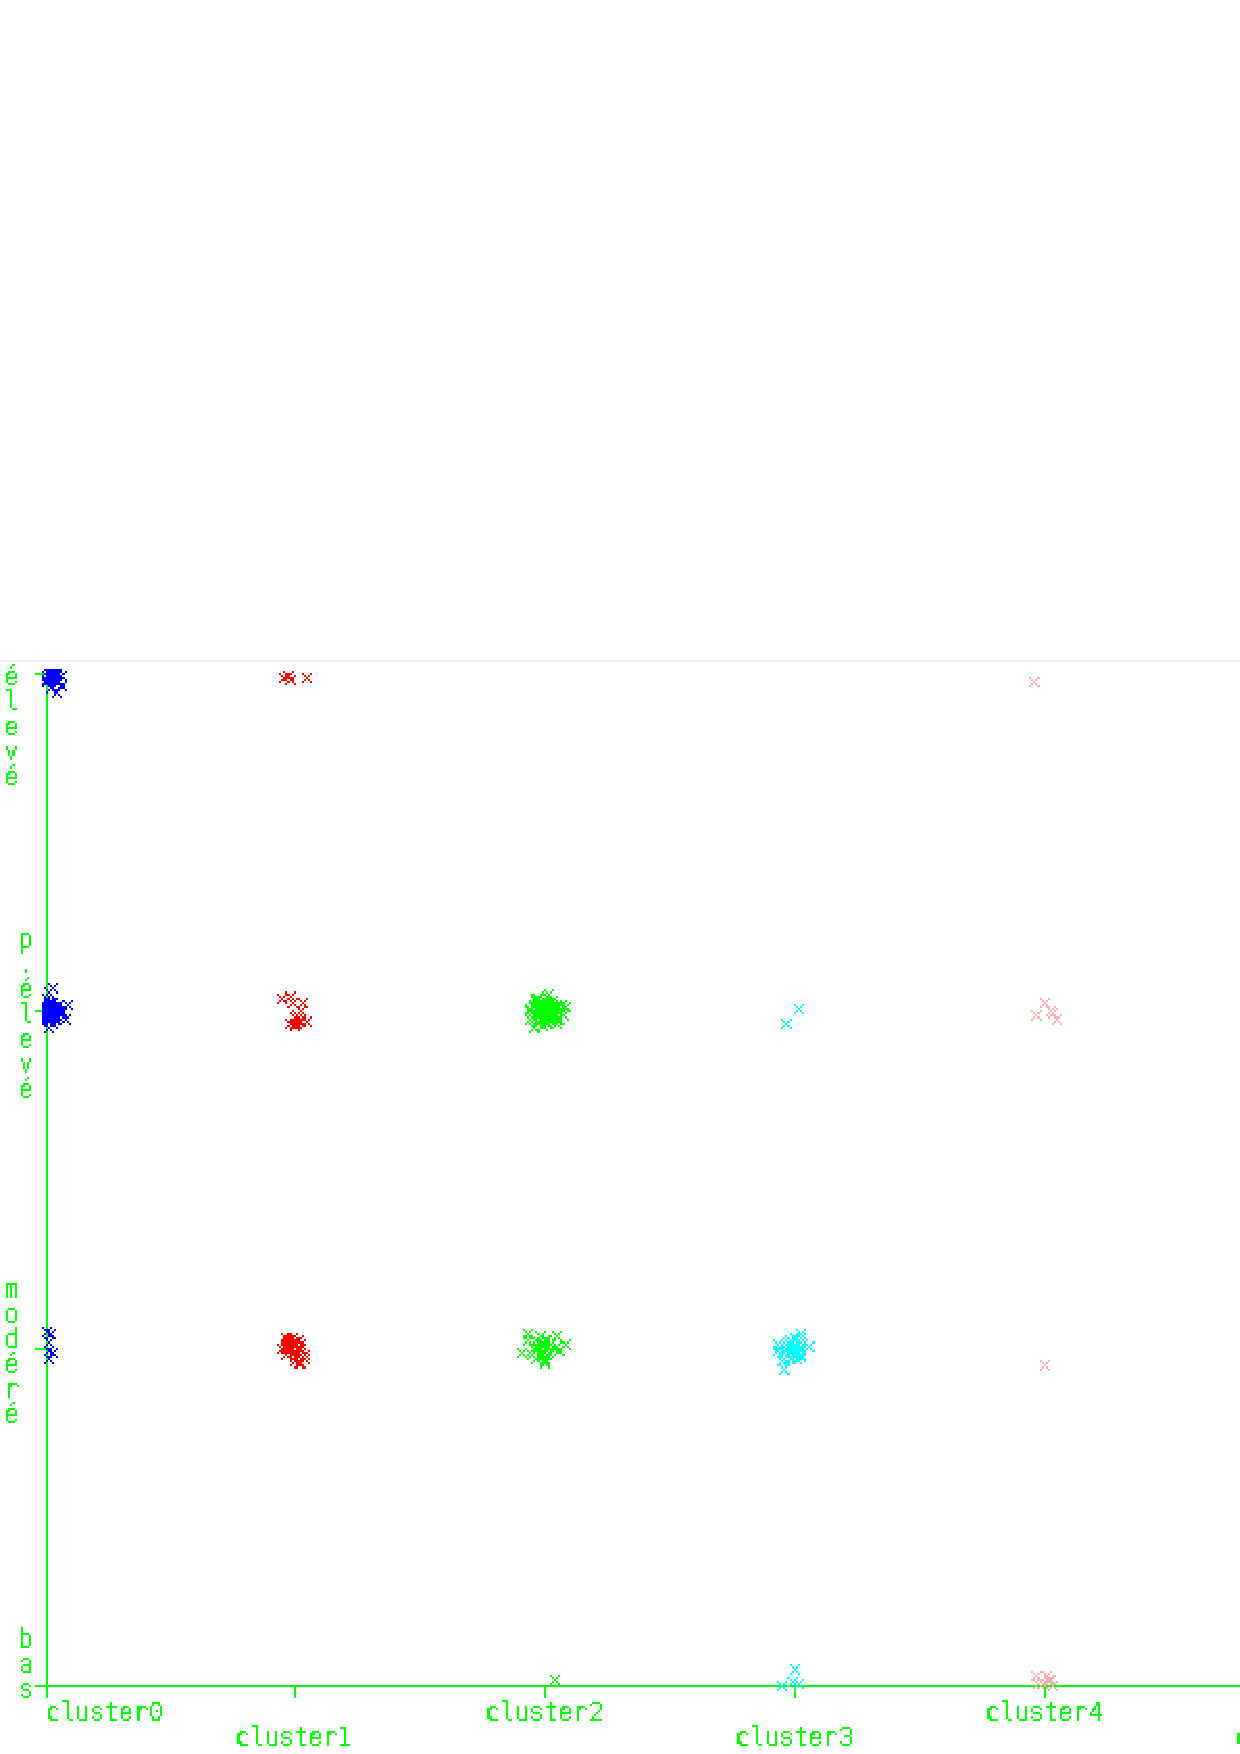
\includegraphics[width=\textwidth]{img_013.pdf}
    \caption{Clusters/temp}
    \end{center}	
\end{figure}

\begin{itemize}
\item les clusters $1$, $2$, $6$ et $7$ contiennent des valeurs \textit{modéré} ou \textit{un peu élevé},
\item les clusters $0$ et $5$ contiennent des valeurs \textit{un peu élevé} ou \textit{élevé},
\item les clusters $3$ et $8$ contiennent des valeurs \textit{modéré} ou \textit{bas},
\item le cluster $4$ est assez disparate.
\end{itemize}

\newpage

\begin{figure}[h!]
    \begin{center}
    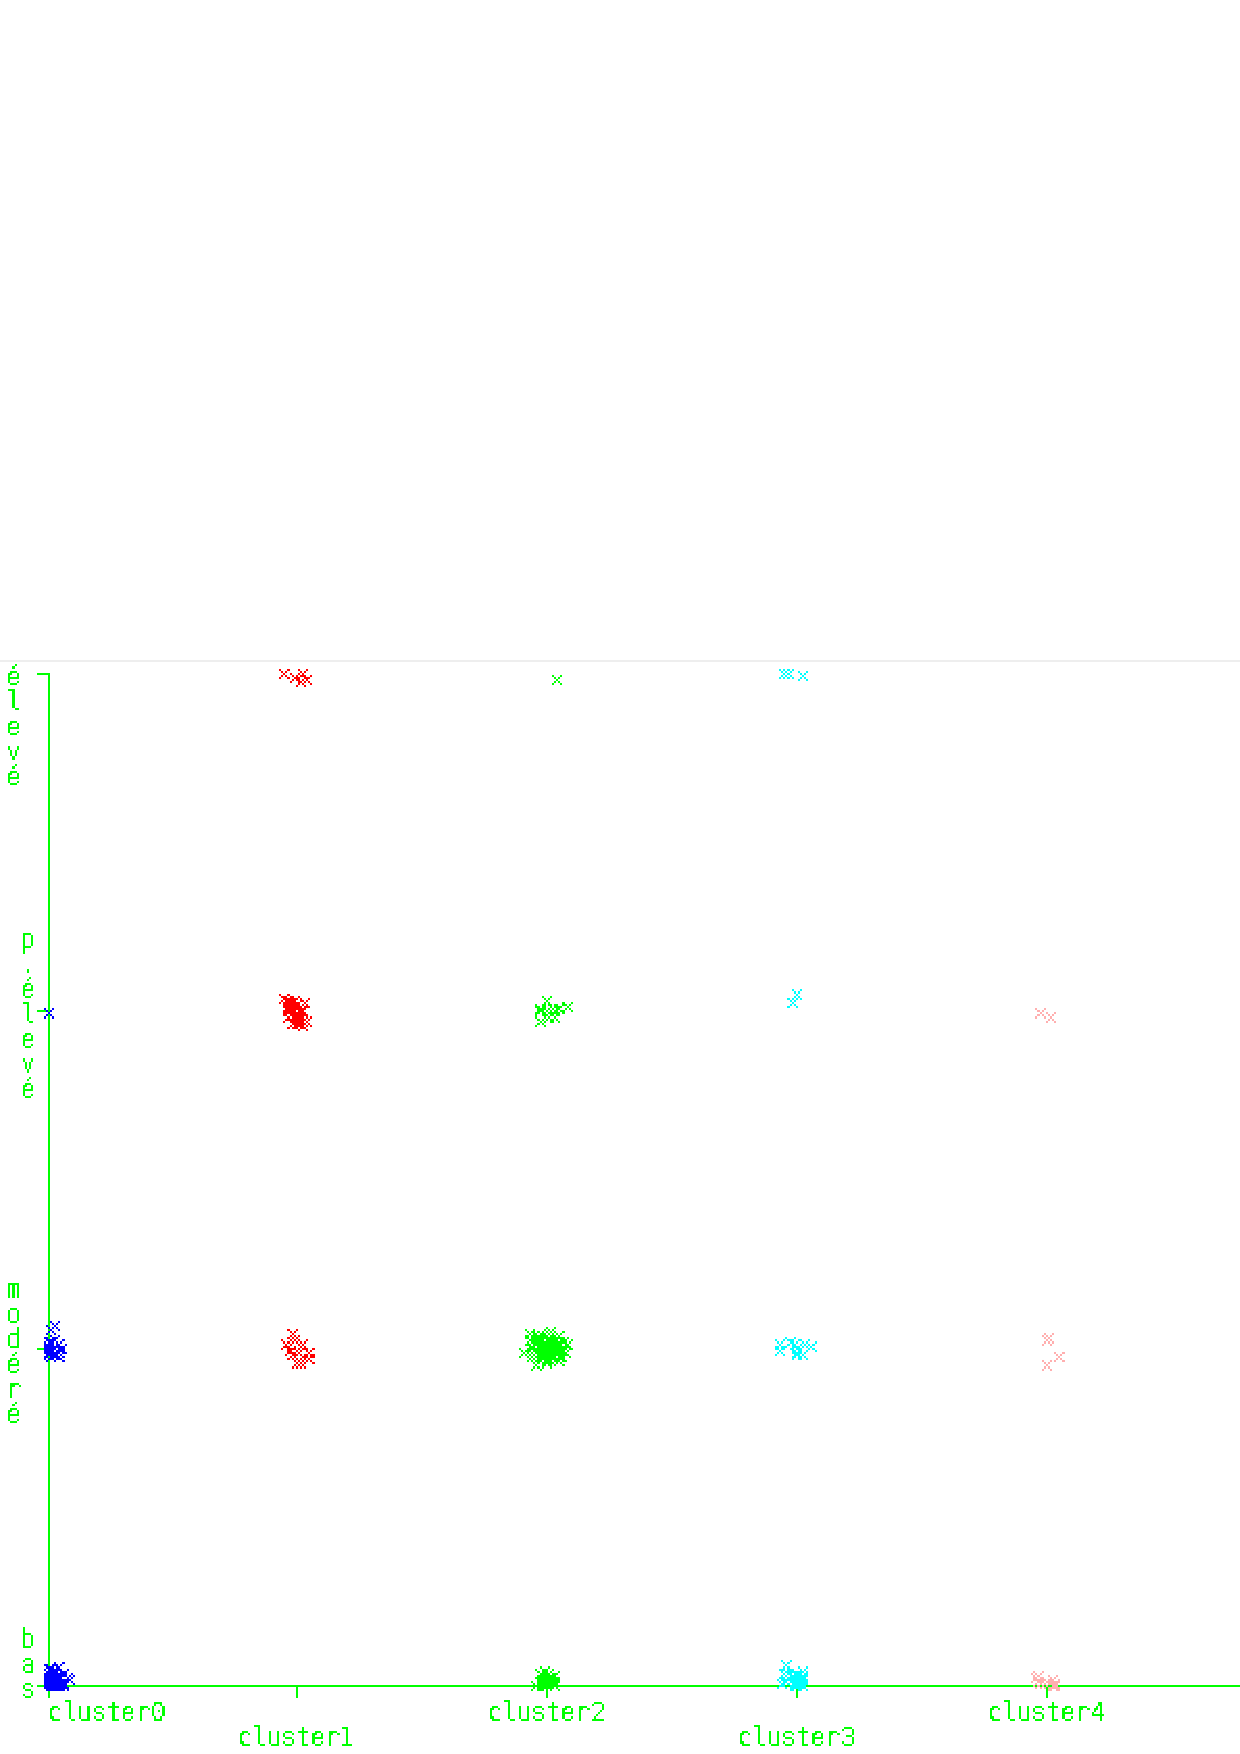
\includegraphics[width=\textwidth]{img_014.pdf}
    \caption{Clusters/RH}
    \end{center}	
\end{figure}

Les clusters sont assez disparates, mis à part le $0$ qui contient des valeurs \textit{modéré} ou \textit{bas} et le cluster $1$ des valeurs 
\textit{modéré} ou supérieure.

\begin{figure}[h!]
    \begin{center}
    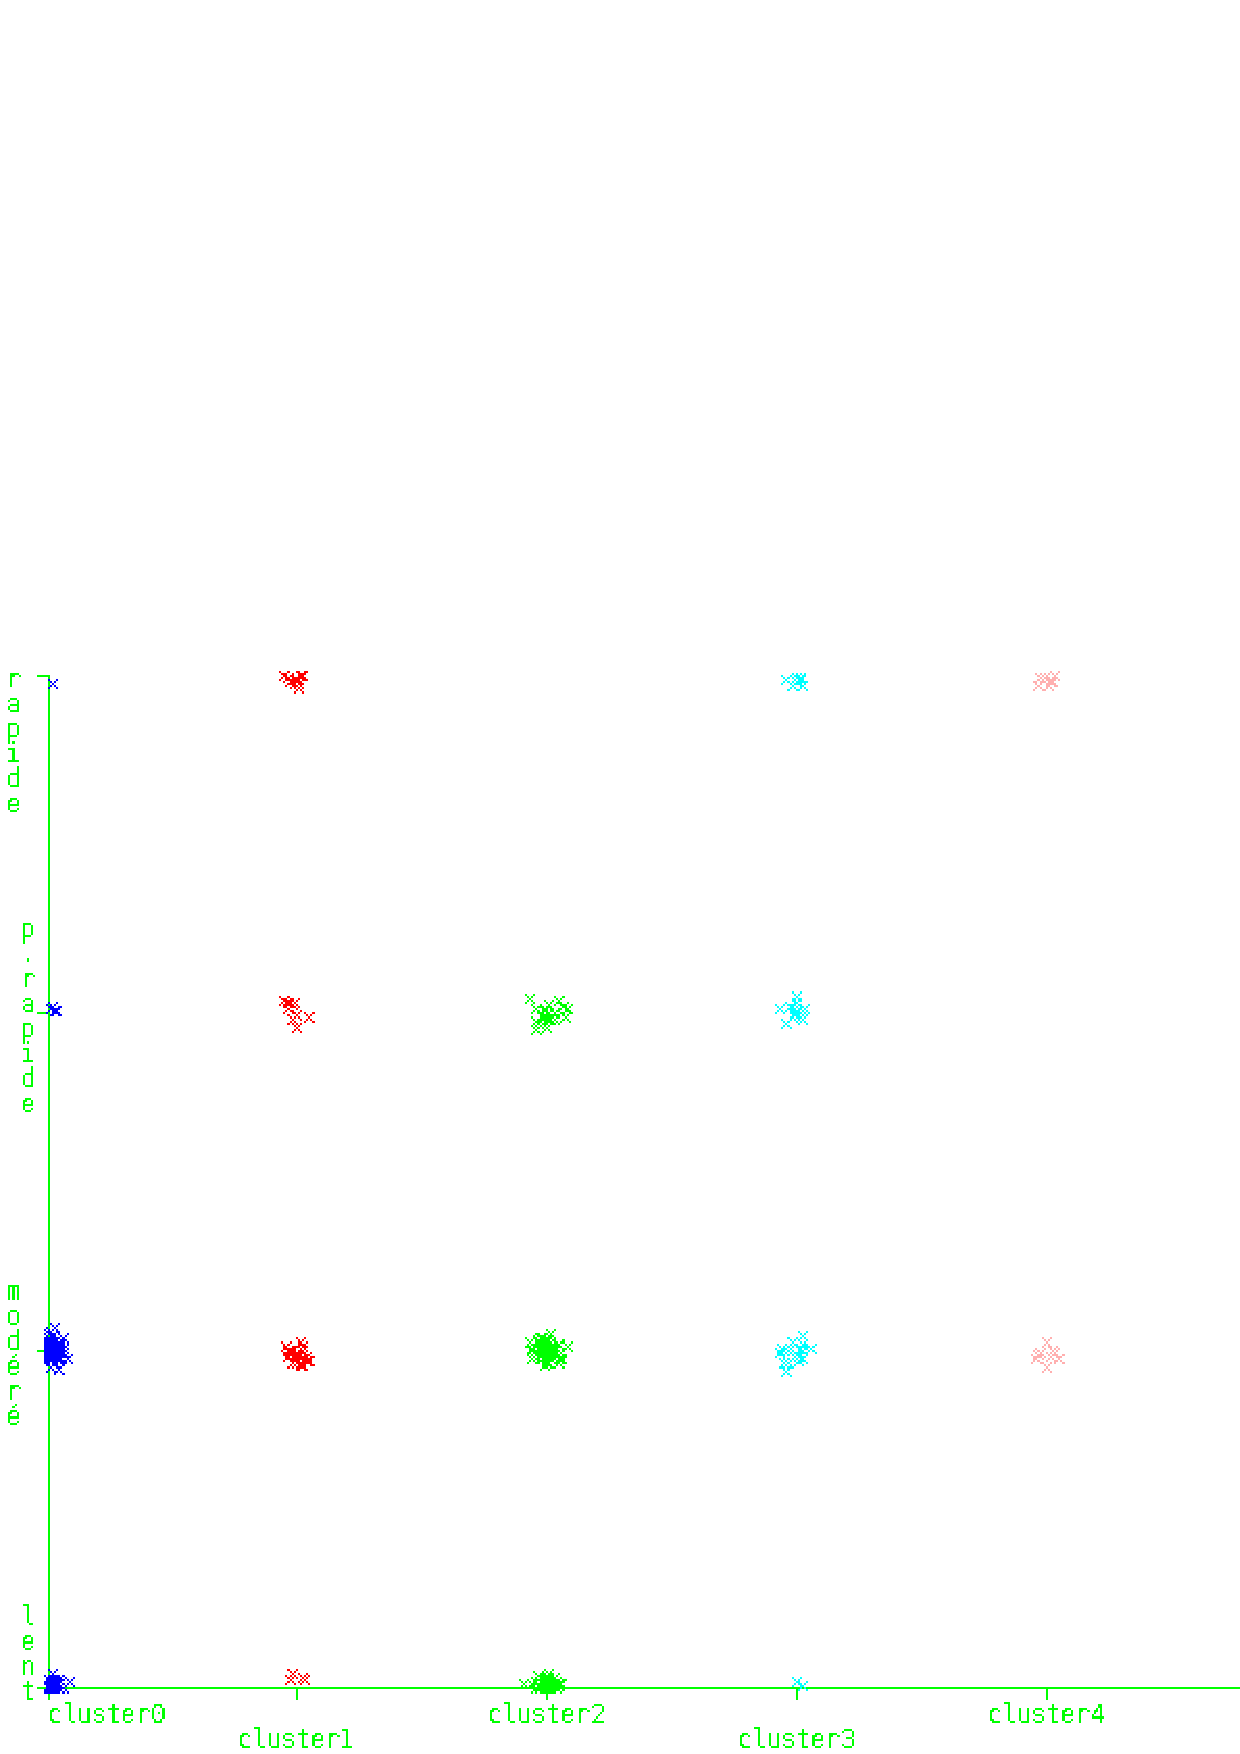
\includegraphics[width=\textwidth]{img_015.pdf}
    \caption{Clusters/wind}
    \end{center}	
\end{figure}

Les clusters $2$ et $5$ ont des valeurs \textit{peu rapide} ou inférieure, le $1$ et $3$ ont des valeurs \textit{modérée} ou supérieure, 
les autres sont assez disparates.

\newpage

\begin{figure}[h!]
    \begin{center}
    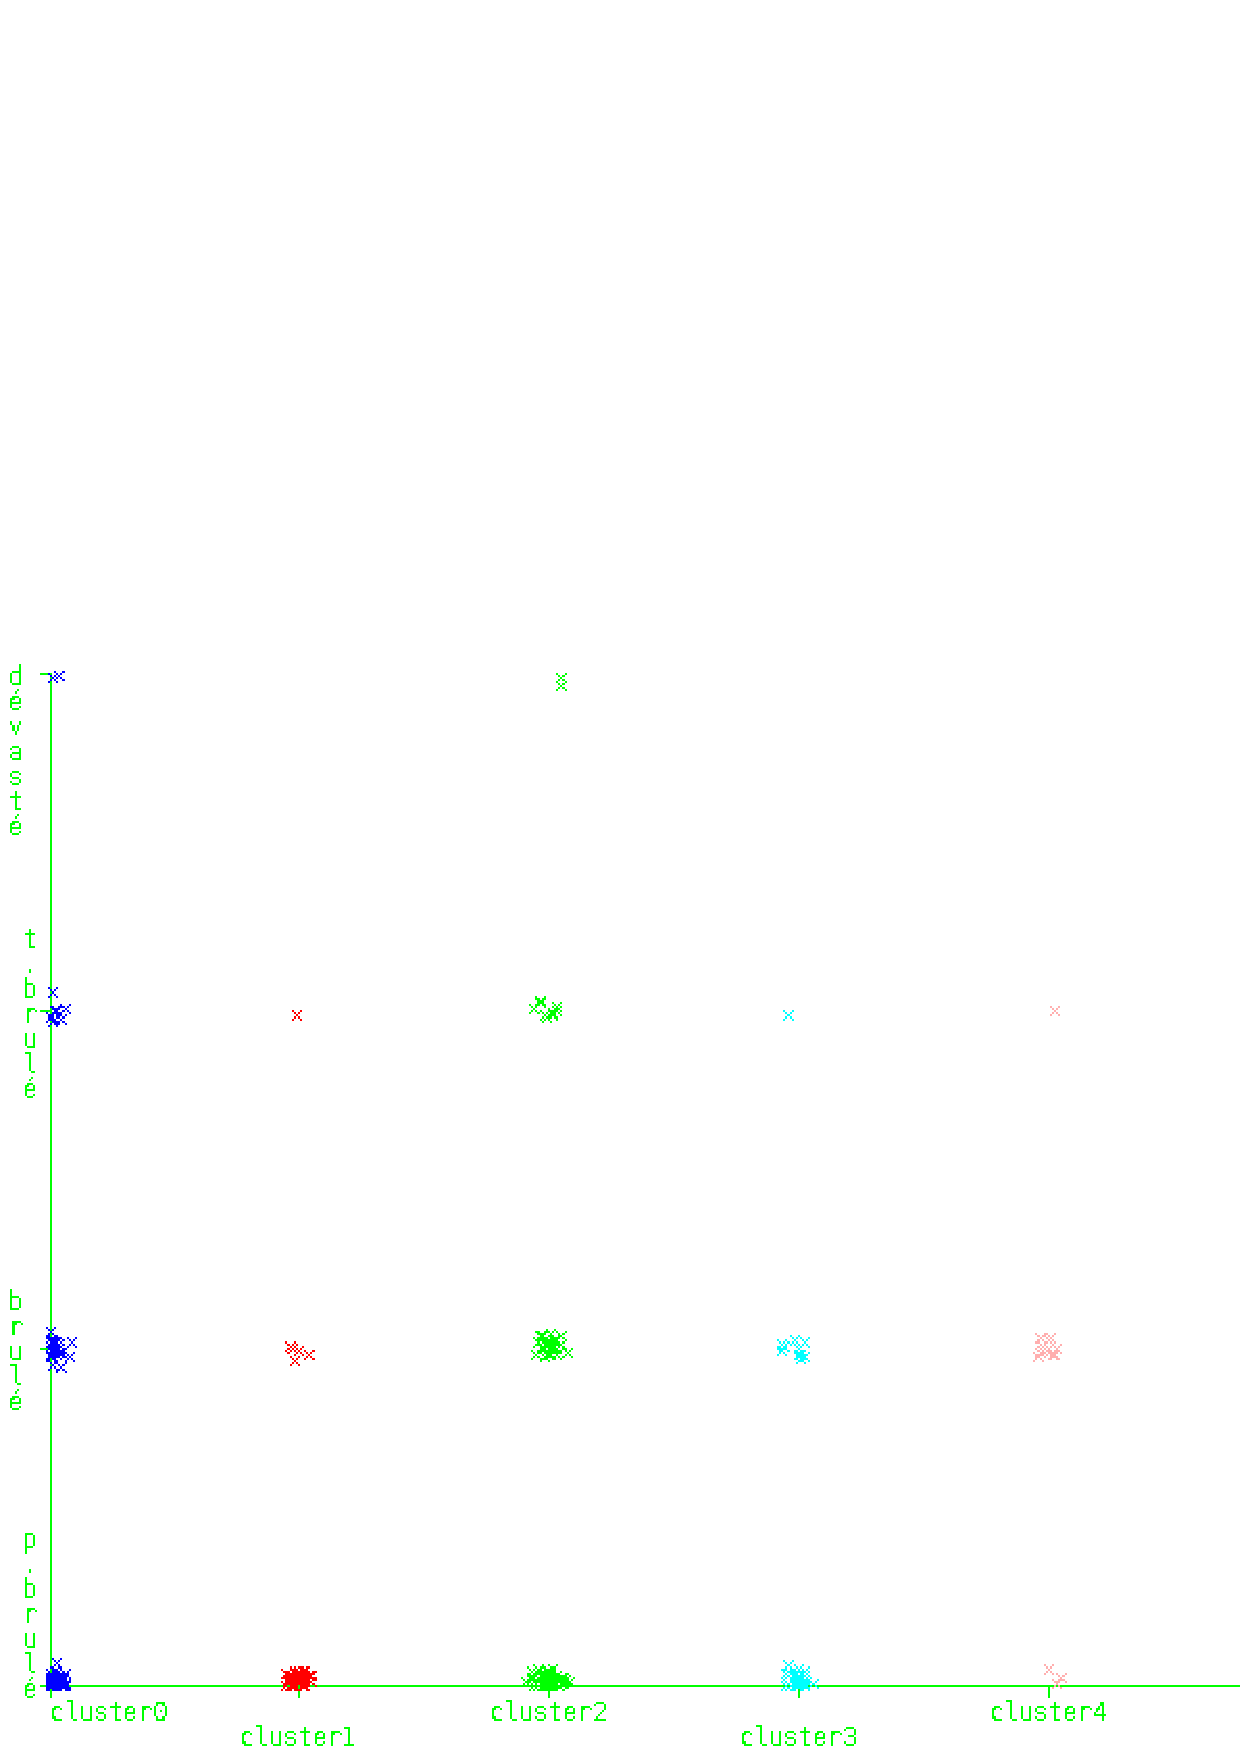
\includegraphics[width=\textwidth]{img_016.pdf}
    \caption{Clusters/area}
    \end{center}	
\end{figure}

Seul le cluster $4$ semble interessant ici, en effet, il s'agit du seul regroupant une majorité de valeur \textit{brulé}, les autres 
regroupant tous en majorité des valeurs \textit{peu brulé}. Remarquons cependant que seuls les clusters $0$, $2$, $5$ et $6$ ont des 
valeurs \textit{dévasté}. \\

Récapitulons les observations que l'on a fait pour les différents clusters et attributs :

\begin{figure}[h!]
    \begin{center}
    \label{t31}
    \begin{tabular}{|c|c|c|c|c|c|c|c|}
    \hline
    Cluster $n^\circ$ & \textbf{season} & \textbf{day} & \textbf{FFMC} & \textbf{DMC} & \textbf{DC} & \textbf{ISI} & \textbf{temp} \\
    \hline
    0 & \firebrick{summer} & \textit{disparate} & \rouge{élevé} & $\geq$ \forest{modéré} & $\geq$ \firebrick{p.élevé} &
	$\geq$ \forest{modéré} & $\geq$ \firebrick{p.élevé}\\
    \hline
    1 & \firebrick{summer} & \firebrick{week-end} & \firebrick{p.élevé} & $\geq$ \forest{modéré} & $\geq$ \firebrick{p.élevé} & 
    \forest{modéré} & \forest{mod}-\firebrick{p.élevé}\\
    \hline
    2 & \firebrick{summer} & \textit{disparate} & \firebrick{p.élevé} & \textit{disparate} & $\geq$ \forest{modéré} & 
    \rouge{$\leq$} \forest{modéré} & \forest{mod}-\firebrick{p.élevé}\\
    \hline
    3 & \blu{winter} & \textit{disparate} & \firebrick{p.élevé} & \blu{bas} & \blu{bas} &
    \forest{modéré} & \rouge{$\leq$} \forest{modéré}\\
    \hline
    4 & \forest{autumn} & \blu{weekday} & \forest{modéré} & \blu{bas} & \textit{disparate} &
    \blu{bas} & \textit{disparate}\\
    \hline
    5 & \firebrick{summer} & \textit{disparate} & \forest{modéré} & $\geq$ \forest{modéré} & $\geq$ \forest{modéré} &
    \firebrick{p.élevé} & $\geq$ \firebrick{p.élevé}\\
    \hline
    6 & \firebrick{summer} & \textit{disparate} & \firebrick{p.élevé} & $\geq$ \forest{modéré} & $\geq$ \forest{modéré} &
    \rouge{$\leq$} \firebrick{p.élevé} & \forest{mod}-\firebrick{p.élevé}\\
    \hline
    7 & \firebrick{summer} & \textit{disparate} & \rouge{élevé} & $\geq$ \forest{modéré} & $\geq$ \forest{modéré} & 
    $\geq$ \firebrick{p.élevé} & \forest{mod}-\firebrick{p.élevé}\\
    \hline
    8 & \blu{winter} & \textit{disparate} & \forest{modéré} & \blu{bas} & \blu{bas} &
    \blu{bas} & \rouge{$\leq$} \forest{modéré}\\
    \hline
    \end{tabular}
    $ $ \\$ $\\$ $\\
    \begin{tabular}{|c|c|c|c|}
    \hline
    Cluster $n^\circ$ & \textbf{RH} & \textbf{wind} & \textbf{area} \\
    \hline
    0 & \rouge{$\leq$} \forest{modéré} & \rouge{$\leq$} \forest{modéré} & \textit{disparate}\\
    \hline
    1 & $\geq$ \forest{modéré} & $\geq$ \forest{modéré} & \rouge{$\leq$} \forest{brulé}\\
    \hline
    2 & \textit{disparate} & \rouge{$\leq$} \firebrick{p.rapide} & \textit{disparate}\\
    \hline
    3 & \textit{disparate} & \textit{disparate} & \rouge{$\leq$} \forest{brulé}\\
    \hline
    4 & \textit{disparate} & \textit{disparate} & \forest{brulé}\\
    \hline
    5 & \textit{disparate} & \rouge{$\leq$} \firebrick{p.rapide} & \textit{disparate}\\
    \hline
    6 & \textit{disparate} & \textit{disparate} & \textit{disparate}\\
    \hline
    7 & \textit{disparate} & \textit{disparate} & \rouge{$\leq$} \firebrick{t.brulé}\\
    \hline
    8 & \textit{disparate} & \textit{disparate} & \rouge{$\leq$} \firebrick{t.brulé}\\
    \hline
    \end{tabular}
    \caption{Résultats du clustering avec EM}
    \end{center}
\end{figure}

Grâce à ce tableau on peut tirer quelques petites conclusions en le lisant ligne par ligne, par exemple à partir du cluster numéro $7$ : 
\begin{quotation}
\textit{\quotecolor{{\Huge ``}}En été, si le \textbf{FFMC} est élevé, que le \textbf{DMC} et le \textbf{DC} sont modérés ou plus, que 
l'\textbf{ISI} \\ \indent est un peu élevé ou plus, que la température est modérée voire un peu élevée ; \\
\indent \textbf{alors}, les feux de forêts déclenchés dans ces circonstances là ont des chances d'être conséquents\\
\indent mais pas dévastateurs.\quotecolor{{\Huge ,,}}}
\end{quotation}

\subsection{SimpleKMeans}

L'utilisation de \textbf{SimpleKMeans} avec $9$ clusters n'apporte aucune information supplémentaire. Tout au plus les clusters 
regroupent plus ou moins de données et ne sont pas classés de la même façon, mais il n'était pas très judicieux de l'utiliser. Voici tout 
de même le résultat de son exécution : \\

\begin{center}
	\begin{verbatim}
kMeans
======

Number of iterations: 5
Within cluster sum of squared errors: 1949.0
Missing values globally replaced with mean/mode

Cluster centroids:
                         Cluster#
Attribute    Full Data          0          1          2          3          4          5
                 (505)       (91)       (67)       (53)       (92)       (83)       (40)
========================================================================================
Xcoord               4          4          6          8          7          6          2
YCoord               4          4          4          6          4          4          5
season          summer     summer     summer     summer     summer     winter     summer
day            weekend    weekday    weekday    weekend    weekend    weekend    weekday
FFMC           p.élevé      élevé    p.élevé      élevé    p.élevé    p.élevé    p.élevé
DMC             modéré     modéré     modéré     modéré     modéré        bas     modéré
DC               élevé      élevé      élevé    p.élevé      élevé        bas      élevé
ISI             modéré     modéré     modéré    p.élevé     modéré        bas        bas
temp           p.élevé    p.élevé     modéré    p.élevé    p.élevé     modéré    p.élevé
RH              modéré        bas    p.élevé        bas     modéré     modéré     modéré
wind            modéré       lent     modéré     modéré     modéré     modéré     modéré
area           p.brulé    p.brulé    p.brulé    p.brulé    p.brulé    p.brulé    p.brulé

               Cluster#
      6          7          8
    (17)       (34)       (28)
=============================
      8          2          1
      6          4          5
 summer     summer     summer
weekday    weekday    weekend
p.élevé      élevé      élevé
 modéré     modéré    p.élevé
  élevé    p.élevé      élevé
    bas    p.élevé     modéré
p.élevé    p.élevé      élevé
    bas        bas        bas
   lent     modéré     modéré
  brulé    p.brulé    p.brulé


=== Model and evaluation on test split ===

kMeans
======

Number of iterations: 8
Within cluster sum of squared errors: 1360.0
Missing values globally replaced with mean/mode

Cluster centroids:
                         Cluster#
Attribute    Full Data          0          1          2          3          4          5
                 (333)      (120)       (24)       (48)       (58)       (20)       (21)
========================================================================================
Xcoord               4          4          2          2          1          6          8
YCoord               4          4          4          4          4          5          6
season          summer     summer     winter     summer     summer     winter     summer
day            weekend    weekday    weekend    weekday    weekend    weekday    weekend
FFMC           p.élevé    p.élevé     modéré      élevé    p.élevé    p.élevé      élevé
DMC             modéré     modéré        bas     modéré     modéré        bas    p.élevé
DC               élevé      élevé        bas      élevé      élevé        bas    p.élevé
ISI             modéré     modéré        bas    p.élevé     modéré        bas     modéré
temp           p.élevé    p.élevé     modéré    p.élevé     modéré     modéré    p.élevé
RH              modéré     modéré    p.élevé        bas     modéré     modéré        bas
wind            modéré     modéré     modéré   p.rapide       lent   p.rapide     modéré
area           p.brulé    p.brulé    p.brulé    p.brulé    p.brulé    p.brulé    t.brulé

       6          7          8
    (18)        (5)       (19)
==============================
      4          6          6
      4          5          5
 winter     spring     summer
weekend    weekend    weekday
p.élevé    p.élevé      élevé
    bas        bas    p.élevé
    bas        bas      élevé
 modéré    p.élevé    p.élevé
 modéré     modéré      élevé
    bas        bas        bas
 modéré     rapide     modéré
  brulé    p.brulé    p.brulé

Clustered Instances

0       70 ( 41%)
1       15 (  9%)
2       20 ( 12%)
3       18 ( 10%)
4       12 (  7%)
5       12 (  7%)
6        9 (  5%)
7        1 (  1%)
8       15 (  9%)
	\end{verbatim}
\end{center}

\subsection{Conclusion de la section}

Cet outil a été le plus utile de tous afin d'atteindre le but visé, il permet également de voir de manière très simple les différentes 
situations qui sont les plus propices à des feux de forêts, de gravité faible à élevée.

\section{Conclusion}

Dans ce rapport, j'ai traité un jeu de données regroupant différentes mesures faites sur les lieux d'un feu de forêt dans le parc 
\textbf{Montesinho} au Portugal. Dans ces mesures on peut retrouver différents indices scientifiques du système \textbf{FWI}, la vitesse 
du vent ou encore la température. Toutes ces informations sont groupées à l'aire brulée lors de l'incendie. Le but du rapport était de 
pouvoir dégager un modèle permettant de définir la gravité d'un feu en fonction uniquement des mesures prises. \\

Le jeu de données était assez compliqué à traiter et a nécessité pas mal de prétraitement afin qu'il soit exploitable. La classification 
ne fonctionne pas très bien sur ce jeu de données à cause du grand nombre de données assez proches (été ou feu peu important) ce qui 
donne des classes très majoritaires dans la plupart des attributs. Les règles d'association ont mieux fonctionné et ont permis de dégager 
quelques circonstances propices aux feux de forêts. Au final, le clustering, lui, nous a permis de spécifier dans chaque cas une plage de 
gravité (par exemple "le feu a des chances d'être important mais pas dévastateur"). \\

En conclusion, je dirais qu'il ne faut pas oublier que les données de l'aire ont du être prétraitée via la fonction $\ln{(x+1)}$ et que 
donc les différences entre 2 classes sont plus prononcées que ce que montre les graphiques. Ce rapport m'a permis de me rendre compte que 
le \textit{Datamining} n'est pas qu'un outil commercial et de marketing mais qu'il permet également de poser des modèles pour les 
scientifiques. Il m'a également permis d'ouvrir les yeux et me convaincre que le \textit{Datamining} est une discipline très importante
de nos jours et que son utilité n'est plus à prouver.

\newpage

\appendix

\section{Annexe 1 : règles d'association}

\subsection{Confiance minimale : $0.9$, Support minimal : $0.2$} \label{annexA}

\begin{center}
	\begin{verbatim}
Best rules found:

  1. DMC=modéré DC=élevé 158 ==> season=summer 158    conf:(1)
  2. DC=p.élevé 110 ==> season=summer 110    conf:(1)
  3. DMC=modéré DC=élevé ISI=modéré 109 ==> season=summer 109    conf:(1)
  4. DMC=modéré DC=élevé area=p.brulé 109 ==> season=summer 109    conf:(1)
  5. DMC=modéré DC=élevé temp=p.élevé 105 ==> season=summer 105    conf:(1)
  6. YCoord=4 DMC=modéré 106 ==> season=summer 105    conf:(0.99)
  7. FFMC=élevé DMC=modéré area=p.brulé 102 ==> season=summer 101    conf:(0.99)
  8. FFMC=élevé DMC=modéré 144 ==> season=summer 142    conf:(0.99)
  9. FFMC=élevé DC=élevé 144 ==> season=summer 141    conf:(0.98)
 10. FFMC=élevé DC=élevé area=p.brulé 105 ==> season=summer 102    conf:(0.97)
 11. DMC=modéré temp=p.élevé 173 ==> season=summer 168    conf:(0.97)
 12. FFMC=élevé temp=p.élevé 136 ==> season=summer 132    conf:(0.97)
 13. FFMC=élevé wind=modéré 129 ==> season=summer 125    conf:(0.97)
 14. day=weekend DMC=modéré 127 ==> season=summer 123    conf:(0.97)
 15. DMC=modéré ISI=modéré 157 ==> season=summer 152    conf:(0.97)
 16. DMC=modéré 263 ==> season=summer 254    conf:(0.97)
 17. DC=élevé temp=p.élevé area=p.brulé 116 ==> season=summer 112    conf:(0.97)
 18. DMC=modéré ISI=modéré area=p.brulé 115 ==> season=summer 111    conf:(0.97)
 19. day=weekday DMC=modéré 136 ==> season=summer 131    conf:(0.96)
 20. DMC=modéré wind=modéré 135 ==> season=summer 130    conf:(0.96)
 21. DMC=modéré temp=p.élevé area=p.brulé 125 ==> season=summer 120    conf:(0.96)
 22. DC=élevé temp=p.élevé 168 ==> season=summer 161    conf:(0.96)
 23. DMC=modéré area=p.brulé 190 ==> season=summer 182    conf:(0.96)
 24. day=weekend FFMC=élevé 107 ==> season=summer 102    conf:(0.95)
 25. YCoord=4 temp=p.élevé 106 ==> season=summer 101    conf:(0.95)
 26. DC=élevé wind=modéré area=p.brulé 106 ==> season=summer 101    conf:(0.95)
 27. DMC=modéré RH=modéré 126 ==> season=summer 120    conf:(0.95)
 28. DC=élevé RH=modéré 120 ==> season=summer 114    conf:(0.95)
 29. day=weekend DC=élevé 134 ==> season=summer 127    conf:(0.95)
 30. DC=élevé area=p.brulé 190 ==> season=summer 180    conf:(0.95)
 31. DC=élevé 274 ==> season=summer 259    conf:(0.95)
 32. FFMC=élevé 217 ==> season=summer 205    conf:(0.94)
 33. YCoord=4 DC=élevé 108 ==> season=summer 102    conf:(0.94)
 34. day=weekday DC=élevé 140 ==> season=summer 132    conf:(0.94)
 35. FFMC=p.élevé DMC=modéré 117 ==> season=summer 110    conf:(0.94)
 36. day=weekday FFMC=élevé 110 ==> season=summer 103    conf:(0.94)
 37. DC=élevé wind=modéré 157 ==> season=summer 147    conf:(0.94)
 38. FFMC=élevé area=p.brulé 153 ==> season=summer 143    conf:(0.93)
 39. DC=élevé ISI=modéré 165 ==> season=summer 154    conf:(0.93)
 40. FFMC=élevé RH=bas 118 ==> season=summer 110    conf:(0.93)
 41. DC=élevé ISI=modéré area=p.brulé 112 ==> season=summer 104    conf:(0.93)
 42. day=weekday temp=p.élevé 122 ==> season=summer 113    conf:(0.93)
 43. FFMC=élevé ISI=modéré 122 ==> season=summer 113    conf:(0.93)
 44. temp=p.élevé 257 ==> season=summer 238    conf:(0.93)
 45. day=weekend temp=p.élevé 135 ==> season=summer 125    conf:(0.93)
 46. temp=p.élevé RH=modéré 133 ==> season=summer 123    conf:(0.92)
 47. temp=p.élevé area=p.brulé 186 ==> season=summer 172    conf:(0.92)
 48. FFMC=p.élevé DC=élevé 119 ==> season=summer 109    conf:(0.92)
 49. temp=p.élevé wind=modéré 138 ==> season=summer 125    conf:(0.91)
 50. ISI=modéré temp=p.élevé 143 ==> season=summer 129    conf:(0.9)	
	\end{verbatim}
\end{center}

\subsection{Confiance minimale : $0.7$, Support minimal : $0.2$} \label{annexB}

\begin{center}
	\begin{verbatim}
Best rules found:

  1. DMC=modéré DC=élevé 158 ==> season=summer 158    conf:(1)
  2. DC=p.élevé 110 ==> season=summer 110    conf:(1)
  3. DMC=modéré DC=élevé ISI=modéré 109 ==> season=summer 109    conf:(1)
  4. DMC=modéré DC=élevé area=p.brulé 109 ==> season=summer 109    conf:(1)
  5. DMC=modéré DC=élevé temp=p.élevé 105 ==> season=summer 105    conf:(1)
  6. YCoord=4 DMC=modéré 106 ==> season=summer 105    conf:(0.99)
  7. FFMC=élevé DMC=modéré area=p.brulé 102 ==> season=summer 101    conf:(0.99)
  8. FFMC=élevé DMC=modéré 144 ==> season=summer 142    conf:(0.99)
  9. FFMC=élevé DC=élevé 144 ==> season=summer 141    conf:(0.98)
 10. FFMC=élevé DC=élevé area=p.brulé 105 ==> season=summer 102    conf:(0.97)
 11. DMC=modéré temp=p.élevé 173 ==> season=summer 168    conf:(0.97)
 12. FFMC=élevé temp=p.élevé 136 ==> season=summer 132    conf:(0.97)
 13. FFMC=élevé wind=modéré 129 ==> season=summer 125    conf:(0.97)
 14. day=weekend DMC=modéré 127 ==> season=summer 123    conf:(0.97)
 15. DMC=modéré ISI=modéré 157 ==> season=summer 152    conf:(0.97)
 16. DMC=modéré 263 ==> season=summer 254    conf:(0.97)
 17. DC=élevé temp=p.élevé area=p.brulé 116 ==> season=summer 112    conf:(0.97)
 18. DMC=modéré ISI=modéré area=p.brulé 115 ==> season=summer 111    conf:(0.97)
 19. day=weekday DMC=modéré 136 ==> season=summer 131    conf:(0.96)
 20. DMC=modéré wind=modéré 135 ==> season=summer 130    conf:(0.96)
 21. DMC=modéré temp=p.élevé area=p.brulé 125 ==> season=summer 120    conf:(0.96)
 22. DC=élevé temp=p.élevé 168 ==> season=summer 161    conf:(0.96)
 23. DMC=modéré area=p.brulé 190 ==> season=summer 182    conf:(0.96)
 24. day=weekend FFMC=élevé 107 ==> season=summer 102    conf:(0.95)
 25. YCoord=4 temp=p.élevé 106 ==> season=summer 101    conf:(0.95)
 26. DC=élevé wind=modéré area=p.brulé 106 ==> season=summer 101    conf:(0.95)
 27. DMC=modéré RH=modéré 126 ==> season=summer 120    conf:(0.95)
 28. DC=élevé RH=modéré 120 ==> season=summer 114    conf:(0.95)
 29. day=weekend DC=élevé 134 ==> season=summer 127    conf:(0.95)
 30. DC=élevé area=p.brulé 190 ==> season=summer 180    conf:(0.95)
 31. DC=élevé 274 ==> season=summer 259    conf:(0.95)
 32. FFMC=élevé 217 ==> season=summer 205    conf:(0.94)
 33. YCoord=4 DC=élevé 108 ==> season=summer 102    conf:(0.94)
 34. day=weekday DC=élevé 140 ==> season=summer 132    conf:(0.94)
 35. FFMC=p.élevé DMC=modéré 117 ==> season=summer 110    conf:(0.94)
 36. day=weekday FFMC=élevé 110 ==> season=summer 103    conf:(0.94)
 37. DC=élevé wind=modéré 157 ==> season=summer 147    conf:(0.94)
 38. FFMC=élevé area=p.brulé 153 ==> season=summer 143    conf:(0.93)
 39. DC=élevé ISI=modéré 165 ==> season=summer 154    conf:(0.93)
 40. FFMC=élevé RH=bas 118 ==> season=summer 110    conf:(0.93)
 41. DC=élevé ISI=modéré area=p.brulé 112 ==> season=summer 104    conf:(0.93)
 42. day=weekday temp=p.élevé 122 ==> season=summer 113    conf:(0.93)
 43. FFMC=élevé ISI=modéré 122 ==> season=summer 113    conf:(0.93)
 44. temp=p.élevé 257 ==> season=summer 238    conf:(0.93)
 45. day=weekend temp=p.élevé 135 ==> season=summer 125    conf:(0.93)
 46. temp=p.élevé RH=modéré 133 ==> season=summer 123    conf:(0.92)
 47. temp=p.élevé area=p.brulé 186 ==> season=summer 172    conf:(0.92)
 48. FFMC=p.élevé DC=élevé 119 ==> season=summer 109    conf:(0.92)
 49. temp=p.élevé wind=modéré 138 ==> season=summer 125    conf:(0.91)
 50. ISI=modéré temp=p.élevé 143 ==> season=summer 129    conf:(0.9)
 51. ISI=modéré wind=modéré 144 ==> season=summer 120    conf:(0.83)
 52. ISI=modéré 268 ==> season=summer 218    conf:(0.81)
 53. ISI=modéré area=p.brulé 190 ==> season=summer 154    conf:(0.81)
 54. YCoord=4 area=p.brulé 141 ==> season=summer 114    conf:(0.81)
 55. season=summer RH=bas 139 ==> FFMC=élevé 110    conf:(0.79)
 56. wind=modéré area=p.brulé 184 ==> season=summer 145    conf:(0.79)
 57. day=weekend wind=modéré 132 ==> season=summer 104    conf:(0.79)
 58. day=weekend ISI=modéré 155 ==> season=summer 122    conf:(0.79)
 59. wind=modéré 271 ==> season=summer 213    conf:(0.79)
 60. day=weekday wind=modéré 139 ==> season=summer 109    conf:(0.78)
 61. YCoord=4 197 ==> season=summer 154    conf:(0.78)
 62. day=weekday area=p.brulé 175 ==> season=summer 136    conf:(0.78)
 63. RH=modéré area=p.brulé 165 ==> season=summer 128    conf:(0.78)
 64. area=p.brulé 354 ==> season=summer 271    conf:(0.77)
 65. RH=modéré 221 ==> season=summer 169    conf:(0.76)
 66. day=weekday 248 ==> season=summer 189    conf:(0.76)
 67. season=summer RH=modéré 169 ==> area=p.brulé 128    conf:(0.76)
 68. day=weekend 257 ==> season=summer 194    conf:(0.75)
 69. day=weekend area=p.brulé 179 ==> season=summer 135    conf:(0.75)
 70. RH=modéré 221 ==> area=p.brulé 165    conf:(0.75)
 71. RH=bas 187 ==> season=summer 139    conf:(0.74)
 72. YCoord=4 season=summer 154 ==> area=p.brulé 114    conf:(0.74)
 73. temp=modéré 158 ==> area=p.brulé 116    conf:(0.73)
 74. FFMC=p.élevé area=p.brulé 165 ==> season=summer 121    conf:(0.73)
 75. DMC=modéré ISI=modéré 157 ==> area=p.brulé 115    conf:(0.73)
 76. FFMC=p.élevé ISI=modéré 142 ==> season=summer 104    conf:(0.73)
 77. season=summer DMC=modéré ISI=modéré 152 ==> area=p.brulé 111    conf:(0.73)
 78. FFMC=p.élevé 229 ==> season=summer 167    conf:(0.73)
 79. FFMC=élevé DC=élevé 144 ==> area=p.brulé 105    conf:(0.73)
 80. season=summer RH=modéré 169 ==> temp=p.élevé 123    conf:(0.73)
 81. ISI=modéré temp=p.élevé 143 ==> area=p.brulé 104    conf:(0.73)
 82. season=summer FFMC=p.élevé 167 ==> area=p.brulé 121    conf:(0.72)
 83. temp=p.élevé 257 ==> area=p.brulé 186    conf:(0.72)
 84. season=summer FFMC=élevé DC=élevé 141 ==> area=p.brulé 102    conf:(0.72)
 85. season=summer temp=p.élevé 238 ==> area=p.brulé 172    conf:(0.72)
 86. DMC=modéré temp=p.élevé 173 ==> area=p.brulé 125    conf:(0.72)
 87. DMC=modéré 263 ==> area=p.brulé 190    conf:(0.72)
 88. season=summer ISI=modéré area=p.brulé 154 ==> DMC=modéré 111    conf:(0.72)
 89. FFMC=p.élevé 229 ==> area=p.brulé 165    conf:(0.72)
 90. season=summer day=weekday 189 ==> area=p.brulé 136    conf:(0.72)
 91. season=summer DMC=modéré ISI=modéré 152 ==> DC=élevé 109    conf:(0.72)
 92. season=summer DMC=modéré 254 ==> area=p.brulé 182    conf:(0.72)
 93. YCoord=4 197 ==> area=p.brulé 141    conf:(0.72)
 94. season=summer DMC=modéré temp=p.élevé 168 ==> area=p.brulé 120    conf:(0.71)
 95. ISI=modéré temp=p.élevé 143 ==> DMC=modéré 102    conf:(0.71)
 96. season=summer FFMC=élevé area=p.brulé 143 ==> DC=élevé 102    conf:(0.71)
 97. season=summer FFMC=élevé DMC=modéré 142 ==> area=p.brulé 101    conf:(0.71)
 98. season=summer RH=modéré 169 ==> DMC=modéré 120    conf:(0.71)
 99. ISI=modéré 268 ==> area=p.brulé 190    conf:(0.71)
100. FFMC=élevé DMC=modéré 144 ==> area=p.brulé 102    conf:(0.71)
	\end{verbatim}
\end{center}

\end{sffamily}\end{document}